%!TEX program = xelatex
% 完整编译: xelatex -> biber/bibtex -> xelatex -> xelatex
\documentclass[lang=cn,a4paper,newtx]{elegantpaper}
\usepackage{algorithm}
\usepackage{algorithmicx}
\usepackage{algpseudocode}
\usepackage{subfig}
\usepackage{longtable}
\usepackage{lipsum}
\usepackage{makecell}
\usepackage{siunitx}
\usepackage{tikz-timing}
\usepackage{tikz}
\usepackage[table]{xcolor}
% \usepackage[backend=biber,style = gb7714-2015]{biblatex}
\addbibresource{reference.bib} % 参考文献,不要删除
\renewcommand{\listtablename}{表格目录}
\renewcommand{\appendixname}{附录~\Alph{section}}

\lstdefinelanguage{Assembly}{
  morekeywords={ ADD, SUB, MPY, JGZ, JMP, AND, OR,BUT,LOAD,STORE,SHIFTL,SHIFTR,HALT},  % 你可以在这里添加更多汇编指令
  sensitive=true,  % 保证区分大小写
  morecomment=[l]; % 单行注释(以分号开始)
  morestring=[b]",  % 字符串用双引号括起来
}
% Define the style for listings
\lstset{
  language=Verilog,  % 选择使用的语言
  basicstyle=\ttfamily\small,  % 基础字体风格
  keywordstyle=\color{blue}\bfseries,  % 指令的颜色和加粗
  commentstyle=\color{gray},  % 注释的颜色
  stringstyle=\color{red},  % 字符串的颜色
  identifierstyle=\color{purple},  % 标识符的颜色
  backgroundcolor=\color{lightgray!10}, % 背景色
  numbers=left,  % 行号显示在左侧
  stepnumber=1,  % 每行显示一个行号
  numberstyle=\tiny\color{gray},  % 行号的字体样式
  numbersep=5pt,  % 行号与代码之间的间距
  breaklines=true,  % 自动换行
  showstringspaces=false,  % 不显示字符串中的空格
  columns=flexible,  % 调整列宽
  frame=single,  % 在代码块外部加一个框
  framerule=0.5mm,  % 框线宽度
  rulesepcolor=\color{black},  % 分隔线颜色
  captionpos=b,  % 标题位置(b: bottom)
  }


  \tikzset{
  timing/name/.cd,
  I/.style={fill=blue!20},    % IF阶段
  D/.style={fill=green!20},   % ID阶段
  F/.style={fill=red!20},     % FO阶段
  N/.style={fill=yellow!20},  % IND阶段
  E/.style={fill=orange!20},  % EX阶段
  W/.style={fill=purple!20}   % WB阶段
}
% \renewcommand{\refname}{参考文献}
\title{计算机组织与结构II:CPU设计文档}
\author{李勃璘 \\ 吴健雄学院}

\version{1.1}
\date{\zhdate{2025/4/25}}

% 本文档命令
\usepackage{array}
\newcommand{\ccr}[1]{\makecell{{\color{#1}\rule{1cm}{1cm}}}}



\begin{document}

\maketitle
\thispagestyle{empty}
\begin{abstract}

\end{abstract}

% Removed
% \vspace{1cm}

% \textbf{版本更新记录:}

% \begin{longtable*}{|c|c|p{10cm}|}
%   \hline
%   \textbf{版本号} & \textbf{日期} & \textbf{更新内容} \\
%   \hline
%   \endfirsthead

%   \hline
%   \textbf{版本号} & \textbf{日期} & \textbf{更新内容} \\
%   \hline
%   \endhead

%   v1.0 & 2025-03-22 & 初始版本,包含基本 CPU 设计框架,流水线结构,Verilog 实现。 \\
%   \hline
%   v1.1 & 2025-03-29 & 修改 \\

% \end{longtable*}


\newpage
\pagenumbering{roman}
\tableofcontents
\newpage
\listoftables
\newpage
\pagenumbering{arabic}
\section{概述}
中央处理单元(CPU)是计算机系统的核心组件,负责执行程序中的指令并处理数据。它由多个核心部件组成,包括算术逻辑单元(ALU)、控制单元(CU)、寄存器、缓存、总线以及与外部存储和外设的接口。CPU的设计和实现是计算机体系结构的基础,决定了计算机的性能、效率以及可扩展性。随着现代计算机技术的不断发展,CPU的设计已经经历了从单核到多核、从简单指令集到复杂指令集的转变,涉及到流水线、缓存管理、指令调度等多个高级设计问题。

在现代CPU中,指令集架构(ISA)定义了CPU能够识别并执行的指令类型,而ALU则负责执行这些指令中的算术和逻辑运算。控制单元(CU)则根据指令的操作码生成控制信号,协调CPU内部和外部的各个组件进行协作。此外,寄存器和缓存等存储单元在数据处理和存储中起着至关重要的作用。通过高效的设计和优化,CPU能够实现高速的计算和响应能力,从而支持各种计算任务的执行。

本文通过设计一个基于FPGA的简化CPU架构,探索了CPU的基本组成与工作原理。整个项目的设计过程中,从指令集的定义到硬件实现,涵盖了计算机体系结构中的核心概念与技术,旨在帮助深入理解CPU设计的各个方面。


本文接下来的章节安排如下:

第二章将介绍CPU内部架构,即指令集、内部寄存器、ALU、内外总线以及控制单元设计,第三章将主要介绍用户面的设计,包括前端输入指令、指令传入内存、结果显示,第四章是二、三章提出的设计方案的Verilog实现和分模块仿真结果,第五章是该设计的整体仿真结果和在NEXYS 4 DDR FPGA开发板上的测试结果。第六章对该设计进行了总结,并提出一些可改进的方向。另外,附录中还提供了设计的全部Verilog代码和项目地址。

% 文献\cite{timeline}设计并实施了一个基于FPGA的五级流水线MIPS CPU课程项目,通过阶段性进度安排和动手实践,有效提升了学生对计算机体系结构的理解和项目完成率。受该工作的启发,本文针对本项目制定了工作安排如表所示。

\section{CPU结构设计}
\subsection{总体架构}

CPU的总架构(包括内存、外设等)示意图可见图~\ref{fig:CPU}。
\begin{figure}[htbp]
  \centering
  \caption{CPU总体架构}
  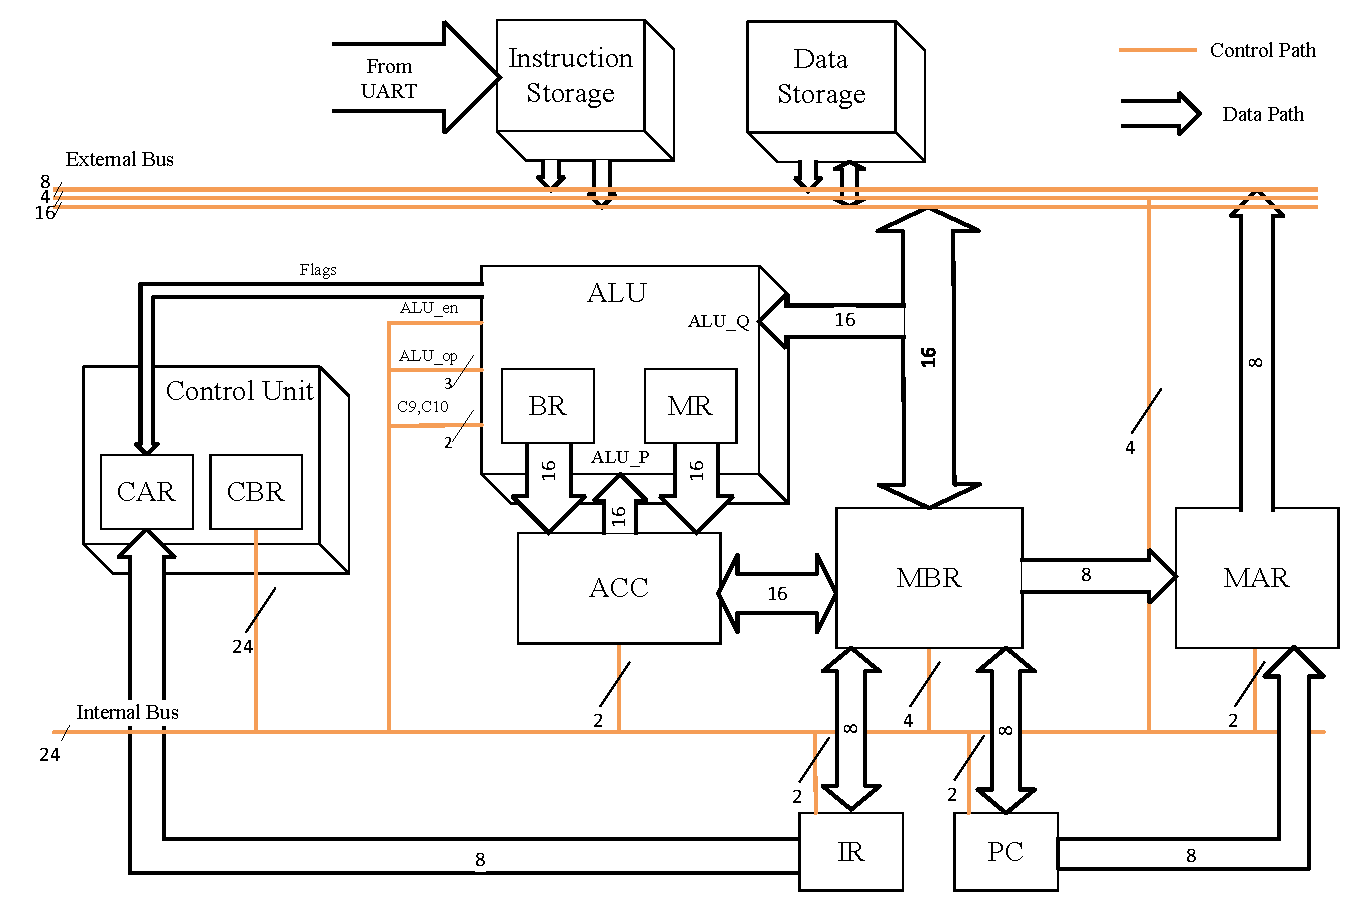
\includegraphics[width = 0.95\textwidth]{figure/CPU_structure.pdf}
  \label{fig:CPU}
\end{figure}

CPU由控制单元(CU),逻辑运算单元(ALU),内存(Memory)和寄存器组(Registers)组成,除内存以外,其余单元由被CU生成的控制信号控制的数据通路(Data Path)连接。另外,MAR和MBR分别还和地址总线、数据总线相连接,用于与内存交互。控制单元和内存都和控制总线相连接,用于与外部控制信号交互。为简单起见,CPU的计算全部为\textbf{16位定点有符号数计算}。





\subsection{指令集架构}
指令集是指CPU能够对数据进行的所有操作的集合。每一条指令都可以被解释为寄存器与寄存器、内存、I/O端口之间的交互。交互方式由CU中的微指令(Micro-operation)给出,且每一条微指令都需要一个时钟执行(如不进行优化)。
\subsubsection{位宽设计}
地址段长为\textbf{8}位,指令码(Opcode)宽度为\textbf{8}位。因此,每一条指令的位宽为\textbf{16}位。


\subsubsection{指令集支持的指令}
指令集共支持13条不同的指令,列于表~\ref{tab:ISA:instructions}。每一条指令包含一个指令码,使用二进制格式存储。
  


\begin{longtable}{c c c}
  \caption{指令集包含指令及功能} \label{tab:ISA:instructions} \\
  \toprule
  助记符  & 指令码(低四位) & 描述 \\
  \midrule
  \endfirsthead
  
  \caption[]{(续表)指令集包含指令及功能} \\
  \toprule
  助记符  & 指令码(低四位) & 描述 \\
  \midrule
  \endhead
  
  \midrule
  \multicolumn{3}{r}{续下页} \\
  \midrule
  \endfoot
  
  \bottomrule
  \endlastfoot
  
  STORE X &  0001   & 结果存入\textbf{数据地址}X \\
  LOAD X  & 0010    & 加载\textbf{数据地址}X \\
  ADD X   & 0011    & 定点数加法\\
  SUB X   & 0100  & 定点数减法\\
  JGZ X   & 0101    & 结果 > 0时跳转至\textbf{指令地址}X\\
  $^\circledast$JMP X   & 0110    & 无条件跳转至\textbf{指令地址}X\\
  HALT    & 0111    & 暂停程序\\
  MPY X   & 1000    & 定点数乘法 \\
  AND X   & 1001    & 按位与\\
  OR X    & 1010    & 按位或\\
  NOT X   & 1011    & 按位非 \\
  SHIFTR X & 1100    & 算术右移 X 位\\
  SHIFTL X & 1101    & 算术左移 X 位\\
\end{longtable}

\subsubsection{寻址方式}
寻址方式指对地址段数据的解释方式。寻址方式由对应指令指定,支持表~\ref{tab:ISA:addressingmode}~中的全部寻址方式。目前设计中指令码的最高位为1时,寻址方式为立即数寻址;指令码的最高位为0时,寻址方式为直接寻址。


\begin{longtable}{c c c}
  \caption{指令集支持的寻址方式} \label{tab:ISA:addressingmode} \\
  \toprule
  寻址方式  & 描述 & 最高位\\
  \midrule
  \endfirsthead
  
  \caption[]{(续表)指令集支持的寻址方式} \\
  \toprule
  寻址方式  & 描述 & 最高位\\
  \midrule
  \endhead
  
  \midrule
  \multicolumn{3}{r}{续下页} \\
  \midrule
  \endfoot
  
  \bottomrule
  \endlastfoot
  
  立即数寻址   &  地址字段是操作数本身,数据为补码格式  & 1\\
  直接寻址 &  地址字段为存放操作数的地址    & 0\\
\end{longtable}

在实际编程中,默认所有指令为\textbf{直接寻址},除非指令中通过标注“IMMEDIATE”明确指定为立即数寻址。详细说明见第~\ref{sec:UserCode}~节。
\subsection{CPU内部寄存器}
该部分描述CPU内部寄存器的含义、存储格式和数据被解释为的格式。这些寄存器通过CPU的内部数据通路相连接。寄存器操作是CPU快速操作的核心。

\begin{longtable}{c c c c c c}
  \caption{CPU内部寄存器的含义、总存储条数、单位位宽和数据解释格式} \label{tab:CPU:datawidth} \\
  \toprule
  寄存器 & 含义 & 条数 & 位宽 & 数据解释格式 & 归属模块\\
  \midrule
  \endfirsthead

  \caption[]{(续表)CPU内部寄存器的含义、总存储条数、单位位宽和数据解释格式} \\
  \toprule
  寄存器 & 含义 & 条数 & 位宽 & 数据解释格式 & 归属模块\\
  \midrule
  \endhead

  \midrule
  \multicolumn{6}{r}{续下页} \\
  \midrule
  \endfoot

  \bottomrule
  \endlastfoot

  PC   & 程序计数器,存储当前指令地址             & 1  & 8   & 指令码(Opcode) & /\\
  MAR  & 内存地址寄存器,存储要访问的内存地址     & 1  & 8   & 地址码(Address)& /\\
  MBR  & 内存缓冲寄存器,存储从内存读取或写入的数据 & 1  & 16  & 二进制补码 & /\\
  IR   & 指令寄存器,存储当前正在执行的指令       & 1  & 8   & 指令码(Opcode)& /\\
  BR   & ALU内部寄存器,存储 ALU 计算结果        & 1  & 16  & 二进制补码 & ALU\\
  ACC  & 累加寄存器,存储 ALU 运算结果           & 1  & 16  & 二进制补码 & /\\
  MR   & ALU内部寄存器,存储 ALU 乘法高 16 位       & 1  & 16  & 二进制补码 & ALU\\
  CM   & 控制存储器,存储微指令控制信号         & 37 & 24  & 控制信号 & CU\\
  CAR  & 控制地址寄存器,指向当前执行的微指令   & 1  & 7   & CM中的条数下标 & CU\\
  CBR  & 控制缓冲寄存器,存储当前微指令的控制信号 & 1  & 24  & 控制信号 & CU\\
\end{longtable}

除上述寄存器以外,ALU进行运算时还会更改\textbf{状态寄存器}(Flags),用于CU进行条件判断。例如,JGZ命令需要判断上一步的运算结果是否大于0,CU便可以直接通过状态寄存器中的ZF(Zero Flag)和NF(Negative Flag)寄存器进行判断。本设计中使用的所有状态寄存器见表~\ref{tab:CPU:status},它们都直接连向CU,通路不受控制信号的控制。Flags对用户公开,配置详见用户交互部分(第~\ref{sec:interaction}~节)。

\begin{longtable}{c c c}
  \caption{状态寄存器列表} \label{tab:CPU:status} \\
  \toprule
  寄存器 & 全称 & 行为 \\ 
  \midrule
  \endfirsthead

  \caption[]{(续表)状态寄存器列表} \\
  \toprule
  寄存器 & 全称 & 行为\\
  \midrule
  \endhead

  \midrule
  \multicolumn{3}{r}{续下页} \\
  \midrule
  \endfoot

  \bottomrule
  \endlastfoot

  ZF   & Zero Flag             & ALU运算结果(通常为ACC)为0时置1\\
  CF  & Carry Flag     & 存储算术移位移出的比特(由于有符号数不存储进位)\\
  OF  & Overflow Flag &  非乘法运算下BR溢出时置1,乘法运算下MR溢出置1\\
  NF  & Negative Flag &  ALU运算结果为负数时置1\\
  MF & Multiply Flag & 乘法运算结果超过16位,且高位未被读取时置1\\
\end{longtable}
\subsection{算术逻辑单元ALU}
算术逻辑单元ALU负责进行大部分CPU内的计算\footnote{自增与PC赋值在设计中不引入ALU。}。

ALU与外围寄存器的控制通路见第~\ref{sec:datapath}~节。ALU受到来自控制单元的$\text{ALU}_{en}$和$\text{ALU}_{op}$控制,前者决定ALU能否进行运算,后者决定ALU执行什么运算。在$\text{ALU}_{en}$为1时,它通过ACC和MBR获取运算的两个数据ALU\_P和ALU\_Q,并将计算结果存入16位BR寄存器(若出现过乘法则可能存入MR寄存器),同时根据LU\_P、ALU\_Q和运算结果和更新Flags寄存器。



表~\ref{tab:aluop}~描述了$\text{ALU}_{op}$与执行运算的对应关系。
\begin{longtable}{c c @{\hskip 2cm} c c}
  \caption{$\text{ALU}_{op}$ 与执行运算的对应关系} \label{tab:aluop} \\
  \toprule
  $\text{ALU}_{op}$ & 运算类型 & $\text{ALU}_{op}$ & 运算类型 \\
  \midrule
  \endfirsthead

  \caption[]{(续表)$\text{ALU}_{op}$ 与执行运算的对应关系} \\
  \toprule
  $\text{ALU}_{op}$ & 运算类型 & $\text{ALU}_{op}$ & 运算类型 \\
  \midrule
  \endhead

  \midrule
  \multicolumn{4}{r}{续下页} \\
  \midrule
  \endfoot

  \bottomrule
  \endlastfoot

  000 & 加法(ADD)       & 100 & 或(OR)         \\
  001 & 减法(SUB)       & 101 & 非(NOT)        \\
  010 & 乘法(MPY)       & 110 & 算术右移(SHIFTR)   \\
  011 & 与(AND)         & 111 & 算术左移(SHIFTL)   \\

\end{longtable}

由于在实际运算中,很可能会出现类似$m\times x +n$的运算。如果加法和减法不支持32位运算,则很可能导致乘法的结果也受溢出影响。因此,设计中引入了MF(Multiply Flag)寄存器,表示乘法运算的结果是否超过16位且未被存储。在MF为1时,加减法被允许进行32位运算,且在16位溢出时不会更新溢出标志位OF。而当出现存储指令STORE时,系统检测到此时MR和BR寄存器都不为0,则会顺次存储BR和MR寄存器(即执行STOREH指令,该指令是一条内部隐藏指令,具体内容见第~\ref{sec:ControlMemory}~节)。由于MR寄存器被读取,MF会被清零,以避免后续的加减法运算受到影响。
% \begin{longtable}{c c c c c c c}
%   \caption{各指令对标志位的影响} \label{tab:ISA:flags} \\
%   \toprule
%   操作码低四位 & 助记符 & ZF & CF & OF & NF & MF\\
%   \midrule
%   \endfirsthead
  
%   \caption[]{(续表)各指令对标志位的影响} \\
%   \toprule
%   操作码低四位 & 助记符 & ZF & CF & OF & NF & MF\\
%   \midrule
%   \endhead
  
%   \midrule
%   \multicolumn{7}{r}{续下页} \\
%   \midrule
%   \endfoot
  
%   \bottomrule
%   \endlastfoot
  
%   0001 & ADD     & 为0时置1 & 0 & 溢出置1 & 负数置1 &\\
%   0010 & SUB     & 为0时置1 & 0 & 溢出置1 & 负数置1 &\\
%   0011 & MPY     & 为0时置1 & 0 & 0 & 负数置1 \\
%   0100 & AND     & 为0时置1 & 0 & 0 & 负数置1 \\
%   0101 & OR      & 为0时置1 & 0 & 0 & 负数置1 \\
%   0110 & NOT     & 为0时置1 & 0 & 0 & 负数置1 \\
%   0111 & SHIFTR  & 为0时置1 & 最低位 & 0 & 负数置1 \\
%   1000 & SHIFTL  & 为0时置1 & 最高位 & 0 & 负数置1 \\

% \end{longtable}
% 放一张表

\subsection{控制单元CU}
控制单元(Control Unit, CU)负责协调和控制寄存器、ALU、内存等各个模块以实现指令的执行。它采用\textbf{微操作指令模式}设计,根据当前指令的操作码和状态寄存器的标志位生成相应的控制信号,指引数据通路中的各个寄存器、ALU、内存和外设进行正确的操作。\ref{sec:cu:structure}~节将介绍该控制单元的结构;\ref{sec:cu:micro}~节将具体描述本设计使用的微操作指令,并提供指令集的微操作指令表以供参考;\ref{sec:datapath}~节将介绍各个控制信号位的作用以及微操作指令表与控制信号的对应。

\subsubsection{控制单元结构}\label{sec:cu:structure}
控制单元由控制地址寄存器(Control Address Register, CAR)、控制数据寄存器(Control Buffer Register, CBR)和控制单元内存(Control Memory, CM)组成,并受到寻址逻辑(Sequencing Logic)的控制。在一个微操作指令周期,控制单元通过完成以下操作执行一个微操作:
\begin{enumerate}
  \item 根据CAR的地址,寻找CM对应地址存储的控制信号,并传输给CBR;
  \item CBR将控制信号译码,传输到相应的接收单元,并将下一跳信息传输给CAR;
  \item 寻址逻辑通过下一跳信息、Flags和Opcode确定下一跳地址,并写入CAR。
\end{enumerate}
控制单元示意图(图~\ref{fig:controlunit})体现了CU内部的关键单元,以及上述操作的数据流向。

\begin{figure}[htbp]
  \centering
  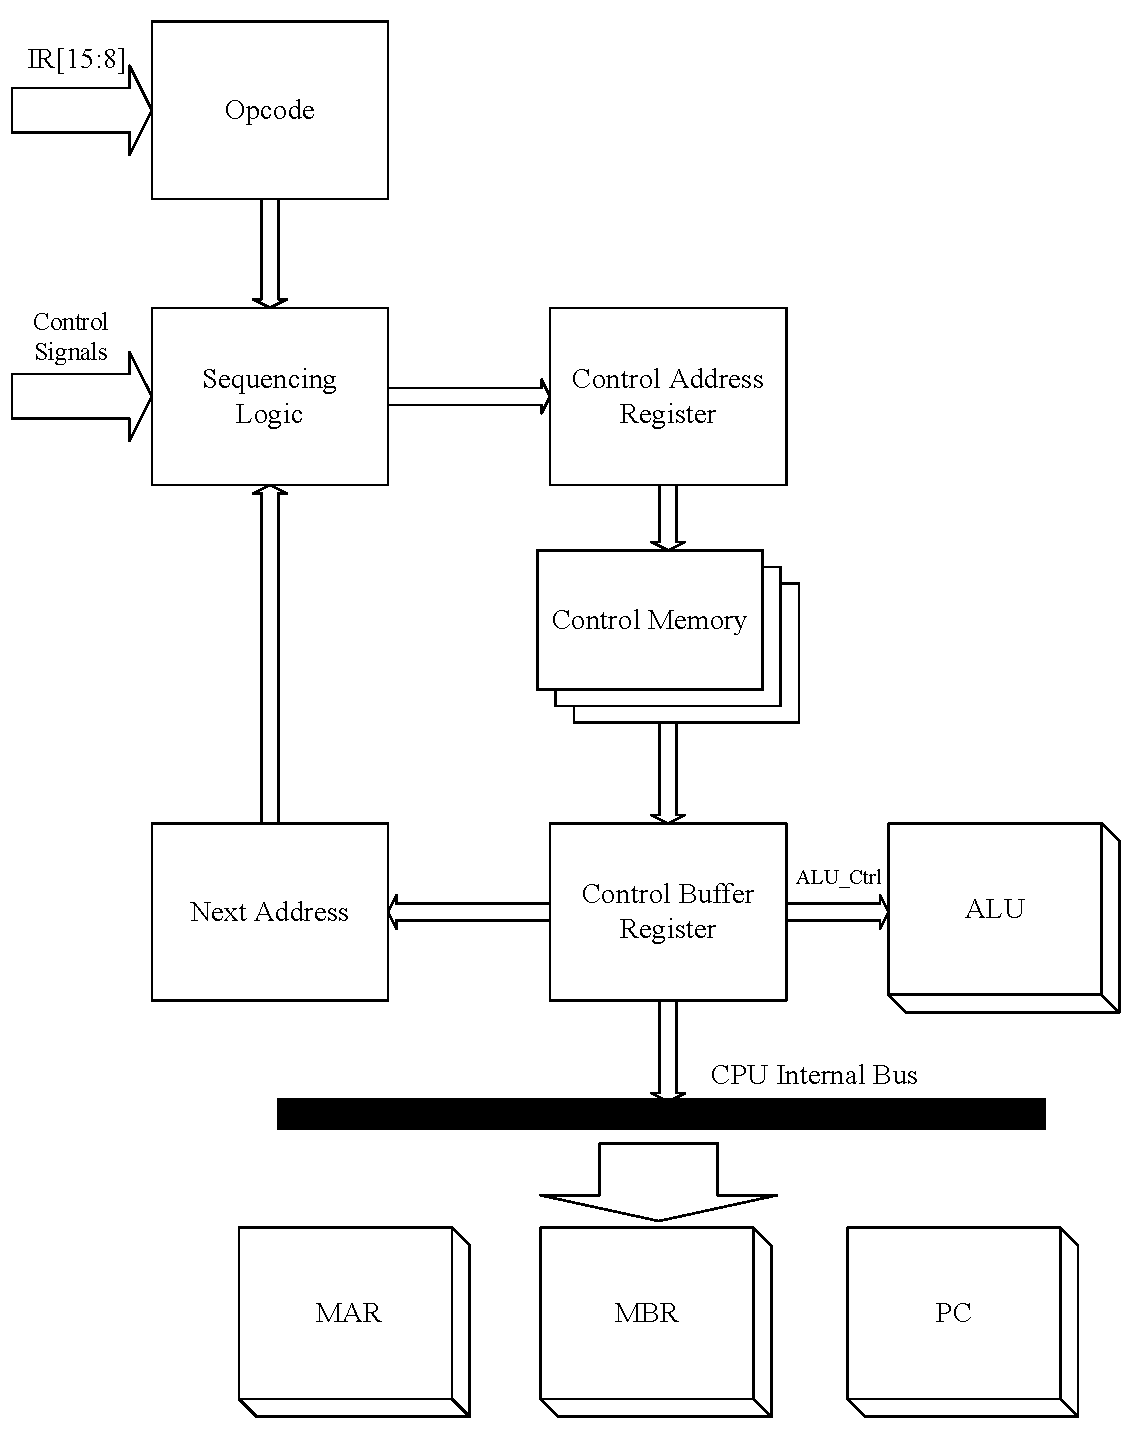
\includegraphics[width = 0.45\textwidth]{figure/CU.pdf}
  \caption{控制单元结构示意图}
  \label{fig:controlunit}
\end{figure}

\subsubsection{微操作指令(Micro-Operations)}\label{sec:cu:micro}
指令集中所有指令都需要多个时钟周期完成,因此需要将指令集的指令分解为多步\textbf{微操作指令}。每步微操作指令通常为寄存器操作。按照寄存器操作的类型,可以将每条指令的执行整合为以下六个步骤,并按步骤顺序执行。
\begin{itemize}
  \item \textbf{IF(Instruction Fetch):}从指令存储器中取出指令,同时确定下一条指令地址(指针指向下一条指令);
  \item \textbf{ID(Instruction Decode):}翻译指令,同时让计算机得出要使用的运算,并得出寻址方式。
  \item \textbf{FO(Fetch Operands):}取立即操作数到MBR,即指令的低8位。
  \item \textbf{IND(Indirect):}间接寻址周期,每插入一个IND周期则间接寻址深度+1。不插入IND周期则为立即数寻址。在本设计中由于不考虑间接寻址,因此最多只有1个IND周期。\textbf{立即数寻址的指令将跳过这一阶段。}
  \item \textbf{EX(Execution):}按照微操作指令指示打开数据通路。
  \item \textbf{WB(Write Back):}将运算结果保存到目标寄存器。
\end{itemize}

注意到:对于所有的指令,前四个阶段的微操作指令是通用的,因此对每一条指令而言,只需要设计EX阶段和WB阶段的微操作指令即可,这大大缩小了CM所需空间。经设计,所有的微操作指令列举于表~\ref{tab:five_stage_pipeline}。

\begin{longtable}{cccc}
  \caption{CPU微操作指令表} \label{tab:five_stage_pipeline}\\
  \toprule
  指令 & 机器码  & EX & WB \\
  \midrule
  \endfirsthead

  \toprule
  \caption[]{(续表)CPU微操作指令表} \\
  \toprule
  指令 & 机器码 & EX & WB \\
  \midrule
  \endhead

  \bottomrule
  \endlastfoot
  \rowcolor{red!10}
  IF & \textbf{阶段} & \multicolumn{2}{c}{$t_1$:MAR ← PC; $t_2$: MBR ← Mem[MAR], PC ← PC+1} \\
  \midrule
  \rowcolor{yellow!10}
  ID & \textbf{阶段} & \multicolumn{2}{c}{$t_1$:IR ← MBR; $t_2$: CU ← IR}\\
  \midrule
  \rowcolor{blue!10}
  FO & \textbf{阶段} & \multicolumn{2}{c}{MBR ← IR[7:0]} \\
  \midrule
  \rowcolor{green!10}
  
  IND & \textbf{阶段} & \multicolumn{2}{c}{$t_1$:MAR ← MBR;  $t_2$:MBR ← Mem[MAR]}\\
  \midrule
  STORE X & 0001  & MAR ← MBR; & Mem[MAR] ← ACC \\

  LOAD X & 0010 &
  无操作 & 
  ACC ← MBR \\
  \midrule
  ADD X & 0011 &
  
  BR ← ACC + MBR & 
  ACC ← BR \\

  SUB X & 0100 &
  
  BR ← ACC - MBR & 
  ACC ← BR \\
  MPY X & 1000 &
  
  MR, BR ← ACC × MBR &
  ACC ← BR \\
  \midrule
  JGZ X & 0101 &
   
  判断:ZF=0 且 NF=0? & 
  \makecell{若满足,PC ← MBR,\\否则 NOP)} \\

  JMP X & 0110 &
  
  无操作 & 
  PC ← MBR \\

  HALT & 0111 &
  
  无操作 & 
  停止程序 \\

  
  \midrule
  AND X & 1001 &
  
  BR ← ACC AND MBR &
  ACC ← BR \\

  OR X & 1010 &
  
  BR ← ACC OR MBR &
  ACC ← BR \\

  NOT X & 1011 &

  BR ← NOT MBR &
  ACC ← BR \\

  SHIFTR X & 1100 &
  
  BR ← ACC $\ggg $ X &
  ACC ← BR \\

  SHIFTL X & 1101 &
  
  BR ← ACC $\lll$ X &
  ACC ← BR \\

\end{longtable}
\subsubsection{CU控制信号(Control Signals)}\label{sec:datapath}
采用水平微指令(Horizontal Micro-operation)设计。水平微指令支持并行操作,执行效率高。每一个水平微指令携带\textbf{所有控制信号位}和\textbf{下一个微操作指令地址的寻址方式}。该CPU共有\textbf{24}位控制信号。其中低16位为寄存器控制信号,高8位为控制字。(图~\ref{fig:control_signal_diagram})

\begin{figure}[htbp]
  \centering
  \caption{控制信号示意图}
  \label{fig:control_signal_diagram}
  \begin{tikzpicture}[node distance=1cm]
  
  % 第一行:控制信号位
  \node (C23) [draw, rectangle, minimum width=1cm, minimum height=1cm] {HLT};
  \node (C22) [draw, rectangle, minimum width=1cm, minimum height=1cm, right of=C23] {SHP};
  \node (C21_20) [draw, rectangle, minimum width=1.5cm, minimum height=1cm, right of=C22,xshift = 0.25cm] {ADDR};
  \node (C19)[draw, rectangle, minimum width=1.5cm, minimum height=1cm, right of=C21_20,xshift = 0.5cm] {$\text{ALU}_{en}$};
  \node (C19_16) [draw, rectangle, minimum width=2cm, minimum height=1cm, right of=C19, xshift=0.75cm] {$\text{ALU}_{op}$};
  \node (C15_0) [draw, rectangle, minimum width=6cm, minimum height=1cm, right of=C19_16, xshift=3cm] {REG Control};
  
  % 第二行:位描述
  % \node (above1) [above left of=C23, text width=2cm, align=center] {\small 23};
  \node (above2) [above left of=C22, text width=2cm, align=center] {\small 23};
  \node (above3) [above left of=C21_20, xshift = -0.1cm,text width=2cm, align=center] {\small 22};
  \node (above4) [above left of=C19, xshift = -0.2cm,text width=2cm, align=center] {\small 20};
  \node (above5) [above left of=C19_16, xshift = -0.4cm,text width=2cm, align=center] {\small 19};
  \node (above6) [above left of=C15_0, xshift = -2.4cm,text width=2cm, align=center] {\small 16};
  \node (above7) [above right of=C15_0, xshift = 2.2cm,text width=0.5cm, align=center] {\small 0};
  % 第三行:复用控制信号位
  \node (C2_desc) [below left of=C15_0, yshift=-0.2cm, text width=5cm, align=center] {\small $C_2$(复用): 指令寄存器读、PC自增};
  
  \end{tikzpicture}
  
  
  \end{figure}

  各控制字的意义如下:
\begin{itemize}
  \item HLT(HALT):全局暂停控制字,所有CPU内部单元停止工作。
  \item SHP(Store High Part):存储乘法寄存器高位结果到指定数据内存地址+1。
  \item ADDR(Address):CU内部控制字,共2位,指示下一步的地址为取指(11)/执行(01)/当前地址+1(10)。
  \item $\text{ALU}_{en}$:ALU使能控制字,允许ALU进行运算操作。
  \item $\text{ALU}_{op}$:ALU运算控制字(3位),指示ALU执行的8种运算类型。运算类型编码可见ALU部分。
  \item REG\_Control:寄存器控制信号(16位),每一位代表两个寄存器/总线之间的开关,对应关系见表~\ref{tab:CPU:DataPath}。
  \item $C_2$:复用控制字。除寄存器控制信号的功能外,还指示指令寄存器读、PC自增。
\end{itemize}

关键存储单元之间通过数据通路进行连接。每条数据通路都由一位控制信号控制。控制信号为1时表示通路打开,数据沿指定流向进行传输。
\begin{longtable}{c c c}
  \caption{寄存器控制信号一览} \label{tab:CPU:DataPath} \\
  \toprule
  控制信号位 & 源寄存器/单元  & 目的寄存器/单元   \\
  \midrule
  \endfirsthead

  \caption[]{(续表)数据通路与控制信号一览} \\
  \toprule
  控制信号位 & 源寄存器/单元  & 目的寄存器/单元  \\
  \midrule
  \endhead

  \midrule
  \multicolumn{3}{r}{续下页} \\
  \midrule
  \endfoot

  \bottomrule
  \endlastfoot

  \multicolumn{3}{c}{\textbf{内部总线控制}}\\
  \midrule
  $C_0 $ & MAR   & 地址总线  \\
  $C_1 $ & PC    & MBR  \\
  $C_2 $ & PC    & MAR  \\
  $C_3 $ & MBR   & PC  \\
  $C_4 $ & MBR   & IR  \\
  $C_5 $ & 数据总线 & MBR  \\
  $C_6 $ & MBR   & ALU\_Q \\
  $C_7 $ & ACC   & ALU\_P  \\
  $C_8 $ & MBR   & MAR  \\
  $C_9 $ & BR   & ACC  \\
  $C_{10}$ & MR   & ACC    \\
  $C_{11}$ & MBR   & ACC  \\
  $C_{12}$ & ACC   & MBR  \\
  $C_{13}$ & MBR   & 数据总线  \\
  $C_{14}$ & IR    & CU  \\
  $C_{15}$ & IR[7:0]    & MBR \\
\end{longtable}

由上述的控制信号位设计,便可以将微操作指令一一对应,画出控制信号表(表~\ref{tab:five_stage_pipeline_ctrl})。控制信号表经过整合后写入CM,结合CU的整体结构和合理的寻址设计,便能完成控制单元的设计。整合逻辑和寻址设计由于涉及到具体电路安排,详见模块设计部分,此处从略。
\begin{longtable}{cccc}
  \caption{CPU控制信号表} \label{tab:five_stage_pipeline_ctrl}\\
  \toprule
  指令 & 机器码  & EX & WB \\
  \midrule
  \endfirsthead

  \toprule
  \caption[]{(续表)CPU控制信号表} \\
  \toprule
  指令 & 机器码 & EX & WB \\
  \midrule
  \endhead

  \bottomrule
  \endlastfoot
  \rowcolor{red!10}
  IF & \textbf{阶段} & \multicolumn{2}{c}{$t_1:C_2$, $t_2:C_0$,$C_5$} \\
  \midrule
  \rowcolor{yellow!10}
  ID & \textbf{阶段} & \multicolumn{2}{c}{$t_1:C_4$,  $t_2:C_{14}$}\\
  \midrule
  \rowcolor{blue!10}
  FO & \textbf{阶段} & \multicolumn{2}{c}{$C_{15}$} \\
  \midrule
  \rowcolor{green!10}
  IND & \textbf{阶段} & \multicolumn{2}{c}{$t_1:C_8$, $t_2:C_0,C_5$}\\
  \midrule
  STORE X & 0001   & $C_8$ & $C_0$,$C_{12}$,$C_{13}$ \\

  LOAD X & 0010  & 
  无操作 & 
  $C_{11}$ \\
  \midrule
  ADD X & 0011 &
  
  $C_6$,$C_7$,$\text{ALU}_{en}$,$\text{ALU}_{op}$ & 
  $C_9$ \\

  SUB X & 0100 &
  $C_6$,$C_7$,$\text{ALU}_{en}$,$\text{ALU}_{op}$ & 
  $C_9$ \\
  MPY X & 1000 &
  $C_6$,$C_7$,$\text{ALU}_{en}$,$\text{ALU}_{op}$ &
  $C_9$ \\
  \midrule
  JGZ X & 0101 &
  
  判断:ZF=0 且 NF=0? & 
  \makecell{若满足,$C_3$\\否则 NOP} \\

  JMP X & 0110 &
  
  无操作 & 
  $C_3$ \\

  HALT & 0111 &
  
  无操作 & 
  HLT \\

  
  \midrule
  AND X & 1001 &
  
  $C_6$,$C_7$,$\text{ALU}_{en}$,$\text{ALU}_{op}$ &
  $C_9$ \\

  OR X & 1010 &
  
  $C_6$,$C_7$,$\text{ALU}_{en}$,$\text{ALU}_{op}$ &
  $C_9$ \\

  NOT X & 1011 &
  
  $C_6$,$\text{ALU}_{en}$,$\text{ALU}_{op}$ &
  $C_9$ \\

  SHIFTR X& 1100 &
  $C_6$,$C_7$,$\text{ALU}_{en}$,$\text{ALU}_{op}$ &
  $C_9$ \\

  SHIFTL X& 1101 &
  $C_6$,$C_7$,$\text{ALU}_{en}$,$\text{ALU}_{op}$ &
  $C_9$ \\

\end{longtable}

\subsection{CPU内部总线和外部总线}\label{sec:ExternalControl}
为了实现CU对CPU内部寄存器的控制,所有内部寄存器均连接到CPU内部总线。CU可对CPU内部总线写控制信号,而所有内部寄存器通过读取内部总线中的某一位或几位控制信号,决定打开自身与某寄存器的数据通路。在本设计中,所有的控制信号作用于\textbf{源寄存器},使得在控制信号关时,数据通路上没有来自源寄存器的数据,避免了可能的误读。例如:对于PC寄存器,其向MAR、MBR输出自身数据,并从MBR获取数据,三个行为分别由$C_1$,$C_2$和$C_3$控制,那么PC只需要读取$C_1$,$C_2$,并在它们打开时输出自身寄存器的值。

MAR和MBR寄存器是CPU与内存或外设的交互接口。由表~\ref{tab:CPU:DataPath}~可知:他们连向了地址总线和数据总线,这两根总线合称外部总线。地址总线为\textbf{8}位单向总线,提供CPU(即MAR)到内存的地址传送通路。数据总线为\textbf{16}位双向总线,提供CPU(即MBR)与内存的双向数据通路。

外部总线还负责管理内存的读写以及选择读写内存设备,受到控制信号$C_0$、$C_2$、$C_5$、$C_{13}$的控制,他们被称为“控制总线”。由于指令和数据的物理存储空间不同,外部总线首先需要确定写入/读取的设备。在整个指令执行的流程中,仅IF阶段需要访问指令内存进行寻址,故该判决逻辑可通过复用控制信号的$C_2$完成。CPU读内存时,$C_0$、$C_5$开,故当且仅当两者同开时,总线可向选中的内存发出读信号,内存读地址总线,向数据总线输出相应地址的数据。CPU写内存时,$C_0$、$C_{13}$开,故当且仅当两者同开时,总线可向选中的内存发出写信号,内存读地址总线,读数据总线并存入对应地址。

\section{外围设备}
\subsection{用户端代码解释}\label{sec:UserCode}
目前采用\textbf{用户编写汇编代码}$\to$\textbf{转换为16位机器码}的方式输入指令。用户可在文本编辑器中编写类汇编代码,而解释器负责将其解释为机器码。

以从1加到100的程序举例:
\begin{lstlisting}[language=Assembly]
  LOAD IMMEDIATE 0    ; 初始化累加器为0 → ACC=0
  STORE 1            ; 存储到地址1(SUM变量)
  LOAD IMMEDIATE 1    ; 初始化计数器为1 → ACC=1
  STORE 2            ; 存储到地址2(i计数器)
LOOP: LOAD 0             ; 读取当前累加值 → ACC=SUM
  ADD 1              ; 加上当前计数器值 → ACC=SUM+i
  STORE 1            ; 更新累加值 → SUM=SUM+i
  LOAD 2             ; 读取计数器 → ACC=i
  ADD IMMEDIATE 1    ; 计数器自增 → ACC=i+1
  STORE 2            ; 更新计数器 → i=i+1
  SUB IMMEDIATE 100  ; 比较是否达到100 → ACC=i-100
  JGZ LOOP           ; 如果i<=100(即ACC<=0),继续循环
  HALT
\end{lstlisting}

代码最终将被解释为一串二进制比特流,解释服从:
\begin{itemize}
  \item 地址占1byte,Opcode占1byte;
  \item 含IMMEDIATE关键字的行,Opcode的MSB为1;
  \item 在代码解释的过程中,标签(\texttt{LOOP})应映射到相同行指令的地址;
  \item 第一条指令的地址为1,依次递增。
\end{itemize}

% 拟采用Python语言对用户代码进行处理,处理好的比特流可通过UART串口通信传入FPGA的BRAM。


\subsection{UART 接收与 指令内存 写入设计}

本设计基于 NEXYS 4 DDR 开发板,通过其板载的 UART 接口完成主机与 FPGA 之间的数据传输。该方案无需额外的数据线或 I/O 资源,即可实现对 FPGA 内部 RAM 的程序写入与指令输入,提升了系统的硬件集成度与使用便捷性。

\subsubsection{UART 接收逻辑}

开发板主系统时钟频率为 \SI{100}{\mega\hertz},串口通信波特率设定为 \SI{115200}{bps}。根据 UART 通信协议,每接收 $1$ 位数据所需的时钟周期数为:

\begin{equation}
  \text{CLK\_BAUD} = \frac{\text{CLK\_FREQ}}{\text{BAUD\_RATE}} = \frac{100\,000\,000}{115200} \approx 868
\end{equation}

采用常见的 \textbf{8N1} 格式传输,即每帧包括:

\begin{itemize}
  \item 1 位起始位(Start Bit);
  \item 8 位数据位(Data Bits);
  \item 1 位停止位(Stop Bit)。
\end{itemize}

因此,每帧共 $10$ 位,总计需要约:

\begin{equation}
  \text{CLK\_FRAME} = 10 \times \text{CLK\_BAUD} = 10 \times 868 = 8680\ \text{cycles}
\end{equation}

接收端在每位开始时执行采样,认为超过0.5秒RX端仍无新数据填入时,指令传输完成。CPU会向用户发出提示,指示接收完成。

\subsubsection{数据缓冲与存储结构}

为保证串口数据完整接收,接收模块首先将每帧数据写入异步 FIFO 缓冲区。随后由控制逻辑从 FIFO 中读取数据,并写入开发板内部的块 RAM。

\paragraph{数据写入格式:}

\begin{itemize}
  \item RAM 的每个地址对应两个字节(16 位)数据;
  \item 高字节为操作码(Opcode),低字节为立即数或地址(Operand);
  \item 若当前行含有 \texttt{IMMEDIATE} 关键字,则 Opcode 的最高位(MSB)为 $1$。
\end{itemize}

\paragraph{写入控制规则:}

\begin{itemize}
  \item 每一条指令都为2byte指令,对于没有操作数的情况,将操作数位置补零。
  \item RAM 地址从地址 0 开始顺序写入。
  \item 程序中如含有 \texttt{LOOP} 标签,将在 RAM 地址分配完毕后由软件在解析阶段回填其地址位置。
\end{itemize}

另外,传入FPGA的所有指令将存于单独的指令内存中,与CPU数据内存隔离开来。CPU内存仅存数据,这符合用户编写的直观感受。每条存入内存的数据位宽为16,即每个地址按顺序存放一条指令。地址从1开始依次递增,防止复位时地址位初始化为0导致出错。指令写入在CPU开机之前,写入成功后开发板亮蓝灯。若在CPU运行时没有指令,则开发板亮红灯。

这种方法通过串口实现了简洁的二进制指令数据装载方式,降低了外设复杂性,为后续的控制单元译码与执行单元操作提供了明确的数据支持。


\subsection{数据内存}
数据内存(RAM)存储CPU保存的数据。内存的大小为 512 Byte,每条存入内存的数据位宽为16,共能存入256条数据。数据内存初始为空,起始写入地址为0,采用Little Endian写入方式\footnote{即高位存储于高地址,低位存储于低地址。}。

CPU与数据内存通过三条总线交互,分别为\textbf{控制总线}、\textbf{地址总线}和\textbf{数据总线}。控制总线中的控制信号决定在这个周期中内存的读/写状态,是否向数据总线写入,同步时序等功能。内存通过读取地址总线决定写入内存中的地址,通过读取数据总线决定写入指定地址中的数据。关于总线的具体配置见~\ref{sec:ExternalControl}。


\subsection{用户交互设计}\label{sec:interaction}
该部分描述用户与FPGA的交互接口(按钮、开关等)以及运行状态信息和结果显示的设计。

\paragraph{全局复位}

按下上侧按钮(BTNH)时,CPU触发全局复位信号,所有寄存器和内存数据清空,控制信号复位为初始状态。

\paragraph{运行与停止}

最左侧开关控制CPU的运行状态:
\begin{itemize}
  \item 开启状态:CPU开始执行指令。
  \item 关闭状态:CPU停止运行并保持当前状态。
\end{itemize}
当CPU发出停止信号(HALT)时,右侧LED灯亮红色;当CPU处于运行状态时,右侧LED灯亮蓝色。

\paragraph{运行模式与单步调试模式}

CPU支持两种模式:
\begin{itemize}
  \item \textbf{运行模式}:CPU自动连续执行指令直至停止,适合快速验证结果。
  \item \textbf{单步调试模式}:用户通过按下最中间的按钮(BTNC)控制CPU逐条执行指令。每次执行完一条指令后,CPU暂停,等待用户操作。
\end{itemize}

最右侧开关控制模式选择:
\begin{itemize}
  \item 开启状态:单步调试模式,左侧LED灯亮红色。
  \item 关闭状态:运行模式,左侧LED灯亮蓝色。
\end{itemize}

\paragraph{结果与指令查看}

\begin{itemize}
  \item 按下左侧按钮(BTNL):查看当前运算结果。
  \item 按下右侧按钮(BTNR):查看当前指令码和指令地址。
  \item 按下下侧按钮(BTND):查看当前Flags寄存器的值。
\end{itemize}
\section{核心模块设计}
\subsection{时钟、复位与停止信号}
CPU由\textbf{全局同步时钟}控制,时钟主频为50MHz。除复位信号外,所有控制逻辑与计算逻辑全部在时钟上升沿进行。UART传输部分使用100MHz的时钟主频。

CPU设有\textbf{全局异步复位}信号,低电平有效。当异步复位时,内存中除指令集数据以外所有数据清空,所有寄存器清空,控制信号全部归为断开(0)。

当CPU执行07号指令HALT时,CPU处于\textbf{停止}状态。与复位不同的是,此时所有寄存器不清空,但所有通路断开。解除该状态的唯一方法是全局复位。

\subsection{UART传输与指令内存}
指令写入通过Python脚本(附录~\ref{sec:appendices:python}~)完成,其可以根据用户输出一串UART格式的比特流。用户可通过PC上的串口调试设备连接UART端口进行传输。
\paragraph{模块代码:}
见附录~\ref{sec:appendices:uart}。
\paragraph{功能块基本信息:}
\begin{itemize}
  \item 模块名:\texttt{INSTR\_ROM}
  \item 最新更新日期:\texttt{4.14}
  \item 是否经过测试:是
\end{itemize}

\paragraph{功能块外部接口:}
\begin{longtable}{>{\bfseries}c c c c}
  \caption{指令内存模块外部接口} \\ 
  \toprule
  信号名 & 方向 & 位宽 & 描述 \\
  \midrule
  \endfirsthead

  \multicolumn{4}{l}{\textbf{(续表)指令内存模块外部接口}} \\
  \toprule
  信号名 & 方向 & 位宽 & 描述 \\
  \midrule
  \endhead
  
  \texttt{i\_clk\_uart} & 输入 & 1 & 时钟信号(100MHz) \\
  \texttt{i\_rst\_n} & 输入 & 1 & 全局复位信号 \\
  \texttt{i\_rx} & 输入 & 1 & 绑定至UART接收引脚 \\
  \texttt{i\_addr\_read} & 输入 & 8 & 读RAM地址 \\
  \texttt{o\_instr\_read} & 输出 & 16 & 指令输出信号 \\
  \texttt{o\_instr\_transmit\_done} & 输出 & 1 & 指令完成传入标志 \\
  \texttt{o\_max\_addr} & 输出 & 8 & 最大地址输出 \\
  \bottomrule
\end{longtable}


\subsubsection{UART模块}
\paragraph{模块基本信息:}
\begin{itemize}
  \item 模块名:\texttt{UART}
  \item 最新更新日期:\texttt{4.30}
  \item 是否经过测试:是
\end{itemize}
\paragraph{模块功能:}
将用户输入代码比特流(8N1格式)译码为1字节数据。分频时钟代码见\hyperref[sec:appendices:uart]{clk\_divider.v}。

\paragraph{模块外部接口:}

\begin{longtable}{>{\bfseries}c c c c}
  \caption{UART模块外部接口} \\
  \toprule
  信号名 & 方向 & 位宽 & 描述 \\
  \midrule
  \endfirsthead

  \multicolumn{4}{l}{\textbf{(续表)UART模块外部接口}} \\
  \toprule
  信号名 & 方向 & 位宽 & 描述 \\
  \midrule
  \endhead

  \texttt{i\_clk}   & 输入  & 1      & 分频后的时钟信号 \\
  \texttt{i\_rst\_n} & 输入  & 1      & 全局复位信号 \\
  \texttt{i\_rx}    & 输入  & 1      & UART 接收引脚 \\
  \texttt{o\_data}  & 输出  & 8    & 接收到的一帧数据 \\
  \texttt{o\_valid} & 输出  & 1      & 数据有效标志,高电平表示 \texttt{o\_data} 已生成 \\
  \texttt{o\_clear\_sign}    & 输出   & 1       & 表示UART输入结束(第一次输入结束后0.5秒内无新的输入)\\
  \bottomrule
\end{longtable}

\paragraph{模块行为:}
\begin{itemize}
  \item 当\texttt{i\_rst\_n}为低电平时,模块复位,状态机进入\texttt{IDLE}状态,清空接收寄存器和计数器;
  \item 在\texttt{IDLE}状态下,若\texttt{i\_rx}信号检测到起始位(低电平),状态机进入\texttt{START}状态;
  \item 在\texttt{START}状态下,等待一个波特率周期后进入\texttt{DATA}状态;
  \item 在\texttt{DATA}状态下,按照波特率时钟采样8位数据,依次存入移位寄存器;
  \item 在接收完8位数据后,状态机进入\texttt{STOP}状态,检测停止位(高电平);
  \item 若停止位有效,输出接收到的8位数据到\texttt{o\_data},并将\texttt{o\_valid}置高,表示数据有效;
  \item 若在\texttt{IDLE}状态下超过0.5秒未接收到新数据,\texttt{o\_clear\_sign}置高,表示UART输入结束;
  \item 状态机在完成当前帧的接收后返回\texttt{IDLE}状态,等待下一帧数据。
\end{itemize}
\subsubsection{FIFO模块}
\paragraph{模块基本信息:}
\begin{itemize}
  \item 模块名:\texttt{FIFO}
  \item 最新更新日期:\texttt{4.13}
  \item 是否经过测试:是
\end{itemize}
\paragraph{模块功能:}
异步FIFO,缓存UART数据并处理UART模块和CPU主模块的跨时钟域问题。它将每两个读出的UART数据拼成2字节的指令输出给BRAM。
\paragraph{模块外部接口:}
\begin{longtable}{>{\bfseries}c c c c}
  \caption{FIFO模块外部接口} \\
  \toprule
  信号名 & 方向 & 位宽 & 描述 \\
  \midrule
  \endfirsthead

  \multicolumn{4}{l}{\textbf{(续表)FIFO模块外部接口}} \\
  \toprule
  信号名 & 方向 & 位宽 & 描述 \\
  \midrule
  \endhead

  \texttt{i\_rst\_n}         & 输入  & 1        & 异步复位信号,低有效 \\
  \texttt{i\_clk\_wr}        & 输入  & 1        & 写时钟信号,UART 使用的 100MHz 时钟 \\
  \texttt{i\_valid\_uart}    & 输入  & 1        & 表示当前 UART 输入数据有效 \\
  \texttt{i\_data\_uart}     & 输入  & 8        & UART 接收到的 8 位数据字节 \\
  \texttt{i\_clk\_rd}        & 输入  & 1        & 读时钟信号,使用100MHz 时钟 \\
  \texttt{o\_data\_bram}     & 输出  & 16       & 两个 UART 字节拼接后的数据,写入 BRAM \\
  \texttt{o\_addr\_bram}     & 输出  & 8        & BRAM 写入地址,从 0 开始自增 \\
  \texttt{o\_wr\_en\_bram}   & 输出  & 1        & BRAM 写使能,高电平表示写入有效 \\
  \texttt{o\_fifo\_empty}    & 输出   & 1       & 表示FIFO空(作为输入完成的判据)\\
  \bottomrule
\end{longtable}
\paragraph{模块行为:}
\begin{itemize}
  \item 当\texttt{i\_rst\_n}为低电平时,FIFO复位:
    \begin{itemize}
      \item 写指针\texttt{wr\_ptr\_bin}和读指针\texttt{rd\_ptr\_bin}清零;
      \item FIFO存储器\texttt{fifo\_mem}清空;
      \item 输出信号\texttt{o\_data\_bram}、\texttt{o\_addr\_bram}和\texttt{o\_wr\_en\_bram}复位为0。
    \end{itemize}
  \item 当\texttt{i\_valid\_uart}信号有效时:
    \begin{itemize}
      \item 若FIFO未满(\texttt{!fifo\_full}),将\texttt{i\_data\_uart}写入\texttt{fifo\_mem}中\texttt{wr\_ptr\_bin}指向的地址;
      \item 写指针\texttt{wr\_ptr\_bin}递增,并更新为Gray码\texttt{wr\_ptr\_gray}。
    \end{itemize}
  \item 在读时钟域(\texttt{i\_clk\_rd}):
    \begin{itemize}
      \item 若FIFO非空(\texttt{!fifo\_empty}),从\texttt{fifo\_mem}中\texttt{rd\_ptr\_bin}指向的地址读取数据;
      \item 若当前为第一个字节(\texttt{byte\_flag}为0),将数据存入缓冲区\texttt{data\_buffer};
      \item 若当前为第二个字节(\texttt{byte\_flag}为1),将缓冲区\texttt{data\_buffer}与当前读取的数据拼接为16位数据,输出到\texttt{o\_data\_bram};
      \item 读指针\texttt{rd\_ptr\_bin}递增,并更新为Gray码\texttt{rd\_ptr\_gray};
      \item 输出写使能信号\texttt{o\_wr\_en\_bram},并将地址\texttt{o\_addr\_bram}递增。
    \end{itemize}
  \item 当FIFO为空时,\texttt{o\_fifo\_empty}置高,表示数据传输完成。
\end{itemize}
\paragraph{备注:}

设计思路参照文献\cite{fifo}。

\subsubsection{指令BRAM模块}
\paragraph{模块基本信息:}
\begin{itemize}
  \item 模块名:\texttt{BRAM\_INSTR}
  \item 最新更新日期:\texttt{4.28}
  \item 是否经过测试:否
\end{itemize}
\paragraph{模块功能:}
描述一指令块RAM,可存放256条2byte指令。读写双口,拥有写使能(FIFO传入)。外部设备可通过开读使能信号并传入地址读取对应地址的2byte指令。
\paragraph{模块外部接口:}
\begin{longtable}{>{\bfseries}c c c c}
  \caption{指令BRAM模块外部接口} \\
  \toprule
  信号名 & 方向 & 位宽 & 描述 \\
  \midrule
  \endfirsthead

  \multicolumn{4}{l}{\textbf{(续表)指令BRAM模块外部接口}} \\
  \toprule
  信号名 & 方向 & 位宽 & 描述 \\
  \midrule
  \endhead

  \texttt{i\_clk}          & 输入  & 1        & 系统时钟信号,驱动读写操作 \\
  \texttt{en\_write}       & 输入  & 1        & 写使能信号,高电平时允许将指令写入 BRAM \\
  \texttt{en\_read}        & 输入  & 1        & 读使能信号,高电平时允许外部总线从 BRAM 中读取指令 \\
  \texttt{i\_addr\_write}  & 输入  & 8        & 要写入的指令地址 \\
  \texttt{i\_instr\_write} & 输入  & 16       & 要写入的指令内容 \\
  \texttt{i\_addr\_read}   & 输入  & 8        & 要读取的指令地址 \\
  \texttt{o\_instr\_read}  & 输出  & 16       & 从 BRAM 中读取的指令内容 \\
  \bottomrule
\end{longtable}




\subsection{控制单元}
控制单元由CAR、CBR寄存器和CM(Control Memory)只读模块组成。控制单元通过将存储于CM的微操作指令和控制信号输出至CBR后,再通过内部控制总线输出到各个单元(寄存器、ALU、外部总线)控制整个系统。控制单元每个时钟周期执行一条微操作指令,由表~\ref{tab:five_stage_pipeline}~可知平均每条指令需要执行8条微操作指令,故每条指令约需要8个周期执行完成。
\subsubsection{Control Memory}\label{sec:ControlMemory}
\paragraph{模块基本信息:}
\begin{itemize}
  \item 模块名:\texttt{CONTROL\_MEMORY}
  \item 最新更新日期:\texttt{4.23}
  \item 是否经过测试:否
\end{itemize}
\paragraph{模块功能:}
存储CPU的水平微操作指令,并根据输入的微操作指令地址写出控制信号到CBR。微操作指令表参考表~\ref{tab:five_stage_pipeline_ctrl}~。另外,为了更好地支持乘法后存储高位、跳转补全周期等操作,CM还存储了两条非指令集中的指令:
\texttt{NOP}和\texttt{STOREH}。它们的作用分别是:
\begin{itemize}
  \item \texttt{NOP}:无操作指令,CPU在执行该指令时不进行任何操作。该指令的作用是占位,保证JGZ指令可以和其余指令执行时间相同。
  \item \texttt{STOREH}:存储高位指令,在上一条指令为乘法时,若本次指令为STORE,则在存放ACC寄存器后,继续将MR寄存器的高位通过ACC寄存器存入地址+1位置的内存。该指令的作用是将乘法运算的高位低位结果都存储到内存中。
\end{itemize}
\paragraph{模块外部接口:}
\begin{longtable}{>{\bfseries}c c c c}
  \caption{Control Memory模块外部接口} \\
  \toprule
  信号名 & 方向 & 位宽 & 描述 \\
  \midrule
  \endfirsthead

  \multicolumn{4}{l}{\textbf{(续表)Control Memory模块外部接口}} \\
  \toprule
  信号名 & 方向 & 位宽 & 描述 \\
  \midrule
  \endhead

  \texttt{car}   & 输入  & 7        & 要读取的微操作指令地址 \\
  \texttt{control\_word}  & 输出  & 24       & 从 CM 中读取的控制信号 \\
  \bottomrule
\end{longtable}
\subsubsection{CAR}
\paragraph{模块基本信息:}
\begin{itemize}
  \item 模块名:\texttt{CAR}
  \item 最新更新日期:\texttt{4.23}
  \item 是否经过测试:否
\end{itemize}
\paragraph{模块功能:}
根据CBR反馈的“下一条地址”逻辑、IR Opcode 和 ALU输出Flags,综合判断出下一条指令所在地址。
\paragraph{模块外部接口:}
\begin{longtable}{>{\bfseries}c c c c}
  \caption{CAR模块外部接口} \\
  \toprule
  信号名 & 方向 & 位宽 & 描述 \\
  \midrule
  \endfirsthead

  \multicolumn{4}{l}{\textbf{(续表)Control Memory模块外部接口}} \\
  \toprule
  信号名 & 方向 & 位宽 & 描述 \\
  \midrule
  \endhead

  \texttt{i\_clk}          & 输入  & 1        & 系统时钟信号,驱动读写操作 \\
  \texttt{i\_rst\_n}      & 输入    & 1       & 全局复位\\
  \texttt{i\_ctrl\_CBR}   & 输入  & 8        & 来自CBR的下一跳地址 \\
  \texttt{o\_signal\_read}  & 输出  & 16       & 从 BRAM 中读取的指令内容 \\
  \bottomrule
\end{longtable}
\subsection{内部寄存器和ALU设计}
\subsubsection{ALU}
ALU(Arithmetic Logic Unit)是算术逻辑单元,负责执行CPU中的算术和逻辑运算。

\paragraph{模块基本信息:}
\begin{itemize}
  \item 模块名:\texttt{ALU}
  \item 最新更新日期:\texttt{2025.4.25}
  \item 是否经过测试:是
\end{itemize}

\paragraph{模块功能:}
ALU模块支持以下功能:
\begin{itemize}
  \item 在控制信号\texttt{ctrl\_alu\_en}有效时,根据\texttt{ctrl\_alu\_op}执行指定的运算;
  \item 支持的运算包括加法、减法、乘法、按位与、按位或、按位非、算术左移和算术右移;
  \item 运算结果存储在BR(低16位)和MR(高16位)寄存器中;
  \item 更新状态寄存器(Flags),包括ZF(零标志)、CF(进位标志)、OF(溢出标志)、NF(负数标志)和MF(乘法标志)。
\end{itemize}

\paragraph{模块外部接口:}
\begin{longtable}{>{\bfseries}c c c c}
  \caption{ALU模块外部接口} \\ 
  \toprule
  信号名 & 方向 & 位宽 & 描述 \\ 
  \midrule
  \endfirsthead

  \multicolumn{4}{l}{\textbf{(续表)ALU模块外部接口}} \\ 
  \toprule
  信号名 & 方向 & 位宽 & 描述 \\ 
  \midrule
  \endhead

  \texttt{i\_clk} & 输入 & 1 & 系统时钟信号 \\ 
  \texttt{i\_rst\_n} & 输入 & 1 & 全局复位信号 \\ 
  \texttt{i\_acc\_alu\_p} & 输入 & 16 & ALU的第一个操作数 \\ 
  \texttt{i\_acc\_alu\_q} & 输入 & 16 & ALU的第二个操作数 \\ 
  \texttt{ctrl\_alu\_op} & 输入 & 3 & 运算类型控制信号 \\ 
  \texttt{ctrl\_alu\_en} & 输入 & 1 & ALU使能信号 \\ 
  \texttt{o\_br} & 输出 & 16 & 运算结果的低16位 \\ 
  \texttt{o\_mr} & 输出 & 16 & 运算结果的高16位(仅乘法有效) \\ 
  \texttt{o\_flags} & 输出 & 5 & 状态寄存器(ZF, CF, OF, NF, MF) \\ 
  \texttt{i\_user\_sample} & 输入 & 1 & 用户采样信号 \\ 
  \texttt{o\_mr\_user} & 输出 & 16 & 输出到用户接口的MR寄存器数据 \\ 
  \bottomrule
\end{longtable}

\paragraph{模块行为:}
\begin{itemize}
  \item 当\texttt{i\_rst\_n}为低电平时,BR和MR寄存器复位为\texttt{16'b0},Flags寄存器复位为\texttt{5'b0};
  \item 当\texttt{ctrl\_alu\_en}信号有效时,根据\texttt{ctrl\_alu\_op}执行以下运算:
    \begin{itemize}
      \item \texttt{000}:加法(ADD),结果存入BR;
      \item \texttt{001}:减法(SUB),结果存入BR;
      \item \texttt{010}:乘法(MPY),低16位存入BR,高16位存入MR;
      \item \texttt{011}:按位与(AND),结果存入BR;
      \item \texttt{100}:按位或(OR),结果存入BR;
      \item \texttt{101}:按位非(NOT),结果存入BR;
      \item \texttt{110}:算术右移(SHIFTR),结果存入BR;
      \item \texttt{111}:算术左移(SHIFTL),结果存入BR。
    \end{itemize}
  \item 根据运算结果更新Flags寄存器:
    \begin{itemize}
      \item \texttt{ZF}:结果为0时置1;
      \item \texttt{CF}:移位操作时存储移出的位;
      \item \texttt{OF}:加法或减法溢出时置1;
      \item \texttt{NF}:结果为负数时置1;
      \item \texttt{MF}:乘法运算时置1。
    \end{itemize}
  \item 当\texttt{i\_user\_sample}信号有效时,将MR寄存器的数据输出到\texttt{o\_mr\_user}。
  \item 在其他情况下,BR和MR寄存器保持当前值。
\end{itemize}

\subsubsection{MAR}
MAR(Memory Address Register)是内存地址寄存器,用于存储当前访问的内存地址。它通过地址总线与内存交互,决定内存的读写地址。

\paragraph{模块基本信息:}
\begin{itemize}
  \item 模块名:\texttt{MAR}
  \item 最新更新日期:\texttt{2025.4.25}
  \item 是否经过测试:是
\end{itemize}

\paragraph{模块功能:}
MAR模块支持以下功能:
\begin{itemize}
  \item 在控制信号\texttt{C8}打开时,从MBR寄存器读取地址;
  \item 在控制信号\texttt{C2}打开时,从PC寄存器读取地址;
  \item 在\texttt{ctrl\_mar\_increment}信号有效时,自增地址(用于支持STOREH指令的高位存储操作)。
\end{itemize}

\paragraph{模块外部接口:}
\begin{longtable}{>{\bfseries}c c c c}
  \caption{MAR模块外部接口} \\ 
  \toprule
  信号名 & 方向 & 位宽 & 描述 \\ 
  \midrule
  \endfirsthead

  \multicolumn{4}{l}{\textbf{(续表)MAR模块外部接口}} \\ 
  \toprule
  信号名 & 方向 & 位宽 & 描述 \\ 
  \midrule
  \endhead

  \texttt{i\_clk} & 输入 & 1 & 系统时钟信号 \\ 
  \texttt{i\_rst\_n} & 输入 & 1 & 全局复位信号 \\ 
  \texttt{i\_mbr\_mar} & 输入 & 8 & 从MBR传入的地址 \\ 
  \texttt{i\_pc\_mar} & 输入 & 8 & 从PC传入的地址 \\ 
  \texttt{ctrl\_mar\_increment} & 输入 & 1 & 自增控制信号 \\ 
  \texttt{C2} & 输入 & 1 & 控制信号,允许从PC读取地址 \\ 
  \texttt{C8} & 输入 & 1 & 控制信号,允许从MBR读取地址 \\ 
  \texttt{o\_mar\_address\_bus} & 输出 & 8 & 输出到地址总线的地址 \\ 
  \bottomrule
\end{longtable}

\paragraph{模块行为:}
\begin{itemize}
  \item 当\texttt{i\_rst\_n}为低电平时,MAR寄存器复位为\texttt{8'b0};
  \item 当\texttt{ctrl\_mar\_increment}信号有效时,MAR寄存器的值自增;
  \item 当\texttt{C8}信号有效时,MAR从\texttt{i\_mbr\_mar}读取地址;
  \item 当\texttt{C2}信号有效时,MAR从\texttt{i\_pc\_mar}读取地址;
  \item 在其他情况下,MAR保持当前值。
\end{itemize}
\subsubsection{MBR}
MBR(Memory Buffer Register)是内存缓冲寄存器,用于存储从内存读取或写入的数据。它通过数据总线与内存交互,是内存与CPU之间的数据桥梁。

\paragraph{模块基本信息:}
\begin{itemize}
  \item 模块名:\texttt{MBR}
  \item 最新更新日期:\texttt{2025.4.25}
  \item 是否经过测试:是
\end{itemize}

\paragraph{模块功能:}
MBR模块支持以下功能:
\begin{itemize}
  \item 在控制信号\texttt{C5}打开时,从数据总线读取数据;
  \item 在控制信号\texttt{C13}打开时,将数据写入数据总线;
  \item 在控制信号\texttt{C6}打开时,将数据传输到ALU的ALU\_Q输入端;
  \item 在控制信号\texttt{C8}打开时,将数据传输到MAR寄存器;
  \item 在控制信号\texttt{C11}打开时,将数据传输到ACC寄存器。
\end{itemize}

\paragraph{模块外部接口:}
\begin{longtable}{>{\bfseries}c c c c}
  \caption{MBR模块外部接口} \\ 
  \toprule
  信号名 & 方向 & 位宽 & 描述 \\ 
  \midrule
  \endfirsthead

  \multicolumn{4}{l}{\textbf{(续表)MBR模块外部接口}} \\ 
  \toprule
  信号名 & 方向 & 位宽 & 描述 \\ 
  \midrule
  \endhead

  \texttt{i\_clk} & 输入 & 1 & 系统时钟信号 \\ 
  \texttt{i\_rst\_n} & 输入 & 1 & 全局复位信号 \\ 
  \texttt{i\_data\_bus} & 输入 & 16 & 从数据总线传入的数据 \\ 
  \texttt{o\_data\_bus} & 输出 & 16 & 输出到数据总线的数据 \\ 
  \texttt{o\_alu\_q} & 输出 & 16 & 输出到ALU的ALU\_Q输入端的数据 \\ 
  \texttt{o\_mar} & 输出 & 8 & 输出到MAR寄存器的地址 \\ 
  \texttt{o\_acc} & 输出 & 16 & 输出到ACC寄存器的数据 \\ 
  \texttt{C5} & 输入 & 1 & 控制信号,允许从数据总线读取数据 \\ 
  \texttt{C13} & 输入 & 1 & 控制信号,允许将数据写入数据总线 \\ 
  \texttt{C6} & 输入 & 1 & 控制信号,允许将数据传输到ALU\_Q \\ 
  \texttt{C8} & 输入 & 1 & 控制信号,允许将数据传输到MAR \\ 
  \texttt{C11} & 输入 & 1 & 控制信号,允许将数据传输到ACC \\ 
  \bottomrule
\end{longtable}

\paragraph{模块行为:}
\begin{itemize}
  \item 当\texttt{i\_rst\_n}为低电平时,MBR寄存器复位为\texttt{16'b0};
  \item 当\texttt{C5}信号有效时,MBR从\texttt{i\_data\_bus}读取数据;
  \item 当\texttt{C13}信号有效时,MBR将数据输出到\texttt{o\_data\_bus};
  \item 当\texttt{C6}信号有效时,MBR将数据输出到\texttt{o\_alu\_q};
  \item 当\texttt{C8}信号有效时,MBR将数据输出到\texttt{o\_mar};
  \item 当\texttt{C11}信号有效时,MBR将数据输出到\texttt{o\_acc};
  \item 在其他情况下,MBR保持当前值。
\end{itemize}
\subsubsection{PC}
PC(Program Counter)是程序计数器,用于存储当前指令的地址,并在指令执行后指向下一条指令的地址。

\paragraph{模块基本信息:}
\begin{itemize}
  \item 模块名:\texttt{PC}
  \item 最新更新日期:\texttt{2025.4.25}
  \item 是否经过测试:是
\end{itemize}

\paragraph{模块功能:}
PC模块支持以下功能:
\begin{itemize}
  \item 在控制信号\texttt{C1}打开时,将当前地址传输到MBR寄存器;
  \item 在控制信号\texttt{C2}打开时,自增地址(用于指令取址阶段);
  \item 在控制信号\texttt{C3}打开时,从MBR寄存器读取地址;
  \item 在复位信号有效时,PC寄存器复位为\texttt{8'd1}。
\end{itemize}

\paragraph{模块外部接口:}
\begin{longtable}{>{\bfseries}c c c c}
  \caption{PC模块外部接口} \\ 
  \toprule
  信号名 & 方向 & 位宽 & 描述 \\ 
  \midrule
  \endfirsthead

  \multicolumn{4}{l}{\textbf{(续表)PC模块外部接口}} \\ 
  \toprule
  信号名 & 方向 & 位宽 & 描述 \\ 
  \midrule
  \endhead

  \texttt{i\_clk} & 输入 & 1 & 系统时钟信号 \\ 
  \texttt{i\_rst\_n} & 输入 & 1 & 全局复位信号 \\ 
  \texttt{i\_mbr\_pc} & 输入 & 8 & 从MBR传入的地址 \\ 
  \texttt{C1} & 输入 & 1 & 控制信号,允许将当前地址传输到MBR \\ 
  \texttt{C2} & 输入 & 1 & 控制信号,允许PC自增 \\ 
  \texttt{C3} & 输入 & 1 & 控制信号,允许从MBR读取地址 \\ 
  \texttt{o\_pc\_mar} & 输出 & 8 & 输出到MAR寄存器的地址 \\ 
  \texttt{o\_pc\_mbr} & 输出 & 8 & 输出到MBR寄存器的地址 \\ 
  \texttt{o\_pc\_user} & 输出 & 8 & 输出到用户接口的地址 \\ 
  \bottomrule
\end{longtable}

\paragraph{模块行为:}
\begin{itemize}
  \item 当\texttt{i\_rst\_n}为低电平时,PC寄存器复位为\texttt{8'd1};
  \item 当\texttt{C2}信号有效时,PC寄存器的值自增;
  \item 当\texttt{C3}信号有效时,PC从\texttt{i\_mbr\_pc}读取地址;
  \item 当\texttt{C1}信号有效时,PC将当前地址输出到\texttt{o\_pc\_mbr};
  \item 在其他情况下,PC保持当前值。
\end{itemize}
\subsubsection{IR}
IR(Instruction Register)是指令寄存器,用于存储当前正在执行的指令,并将指令的操作码和操作数分离,供控制单元和其他模块使用。

\paragraph{模块基本信息:}
\begin{itemize}
  \item 模块名:\texttt{IR}
  \item 最新更新日期:\texttt{2025.4.25}
  \item 是否经过测试:是
\end{itemize}

\paragraph{模块功能:}
IR模块支持以下功能:
\begin{itemize}
  \item 在控制信号\texttt{C4}打开时,从MBR寄存器读取指令;
  \item 在控制信号\texttt{C14}打开时,将操作码输出到控制单元(CU);
  \item 在控制信号\texttt{C15}打开时,将操作数输出到MBR寄存器;
  \item 在用户采样信号有效时,将操作码输出到用户接口。
\end{itemize}

\paragraph{模块外部接口:}
\begin{longtable}{>{\bfseries}c c c c}
  \caption{IR模块外部接口} \\ 
  \toprule
  信号名 & 方向 & 位宽 & 描述 \\ 
  \midrule
  \endfirsthead

  \multicolumn{4}{l}{\textbf{(续表)IR模块外部接口}} \\ 
  \toprule
  信号名 & 方向 & 位宽 & 描述 \\ 
  \midrule
  \endhead

  \texttt{i\_clk} & 输入 & 1 & 系统时钟信号 \\ 
  \texttt{i\_rst\_n} & 输入 & 1 & 全局复位信号 \\ 
  \texttt{i\_mbr\_ir} & 输入 & 16 & 从MBR传入的指令 \\ 
  \texttt{C4} & 输入 & 1 & 控制信号,允许从MBR读取指令 \\ 
  \texttt{C14} & 输入 & 1 & 控制信号,允许将操作码输出到CU \\ 
  \texttt{C15} & 输入 & 1 & 控制信号,允许将操作数输出到MBR \\ 
  \texttt{i\_user\_sample} & 输入 & 1 & 用户采样信号 \\ 
  \texttt{o\_ir\_cu} & 输出 & 8 & 输出到CU的操作码 \\ 
  \texttt{o\_ir\_mbr} & 输出 & 8 & 输出到MBR的操作数 \\ 
  \texttt{o\_ir\_user} & 输出 & 8 & 输出到用户接口的操作码 \\ 
  \bottomrule
\end{longtable}

\paragraph{模块行为:}
\begin{itemize}
  \item 当\texttt{i\_rst\_n}为低电平时,IR寄存器复位为\texttt{8'b0};
  \item 当\texttt{C4}信号有效时,从\texttt{i\_mbr\_ir}读取指令,并将高8位存储为操作码,低8位存储为操作数;
  \item 当\texttt{C14}信号有效时,将操作码输出到\texttt{o\_ir\_cu};
  \item 当\texttt{C15}信号有效时,将操作数输出到\texttt{o\_ir\_mbr};
  \item 当\texttt{i\_user\_sample}信号有效时,将操作码输出到\texttt{o\_ir\_user};
  \item 在其他情况下,IR保持当前值。
\end{itemize}
\subsubsection{ACC}
ACC(Accumulator)是累加寄存器,用于存储ALU运算的结果低16位,并作为ALU的输入之一。

\paragraph{模块基本信息:}
\begin{itemize}
  \item 模块名:\texttt{ACC}
  \item 最新更新日期:\texttt{2025.4.25}
  \item 是否经过测试:是
\end{itemize}

\paragraph{模块功能:}
ACC模块支持以下功能:
\begin{itemize}
  \item 在控制信号\texttt{C9}打开时,从BR寄存器读取数据;
  \item 在控制信号\texttt{C10}打开时,从MR寄存器读取数据;
  \item 在控制信号\texttt{C11}打开时,从MBR寄存器读取数据;
  \item 在控制信号\texttt{C12}打开时,将数据传输到MBR寄存器;
  \item 在控制信号\texttt{C7}打开时,将数据传输到ALU的ALU\_P输入端;
  \item 在用户采样信号有效时,将数据输出到用户接口。
\end{itemize}

\paragraph{模块外部接口:}
\begin{longtable}{>{\bfseries}c c c c}
  \caption{ACC模块外部接口} \\ 
  \toprule
  信号名 & 方向 & 位宽 & 描述 \\ 
  \midrule
  \endfirsthead

  \multicolumn{4}{l}{\textbf{(续表)ACC模块外部接口}} \\ 
  \toprule
  信号名 & 方向 & 位宽 & 描述 \\ 
  \midrule
  \endhead

  \texttt{i\_clk} & 输入 & 1 & 系统时钟信号 \\ 
  \texttt{i\_rst\_n} & 输入 & 1 & 全局复位信号 \\ 
  \texttt{i\_br\_acc} & 输入 & 16 & 从BR传入的数据 \\ 
  \texttt{i\_mr\_acc} & 输入 & 16 & 从MR传入的数据 \\ 
  \texttt{i\_mbr\_acc} & 输入 & 16 & 从MBR传入的数据 \\ 
  \texttt{C7} & 输入 & 1 & 控制信号,允许将数据传输到ALU\_P \\ 
  \texttt{C9} & 输入 & 1 & 控制信号,允许从BR读取数据 \\ 
  \texttt{C10} & 输入 & 1 & 控制信号,允许从MR读取数据 \\ 
  \texttt{C11} & 输入 & 1 & 控制信号,允许从MBR读取数据 \\ 
  \texttt{C12} & 输入 & 1 & 控制信号,允许将数据传输到MBR \\ 
  \texttt{i\_user\_sample} & 输入 & 1 & 用户采样信号 \\ 
  \texttt{o\_acc\_alu\_p} & 输出 & 16 & 输出到ALU的ALU\_P输入端的数据 \\ 
  \texttt{o\_acc\_mbr} & 输出 & 16 & 输出到MBR的数据 \\ 
  \texttt{o\_acc\_user} & 输出 & 16 & 输出到用户接口的数据 \\ 
  \bottomrule
\end{longtable}

\paragraph{模块行为:}
\begin{itemize}
  \item 当\texttt{i\_rst\_n}为低电平时,ACC寄存器复位为\texttt{16'b0};
  \item 当\texttt{C9}信号有效时,ACC从\texttt{i\_br\_acc}读取数据;
  \item 当\texttt{C10}信号有效时,ACC从\texttt{i\_mr\_acc}读取数据;
  \item 当\texttt{C11}信号有效时,ACC从\texttt{i\_mbr\_acc}读取数据;
  \item 当\texttt{C12}信号有效时,ACC将数据输出到\texttt{o\_acc\_mbr};
  \item 当\texttt{C7}信号有效时,ACC将数据输出到\texttt{o\_acc\_alu\_p};
  \item 当\texttt{i\_user\_sample}信号有效时,ACC将数据输出到\texttt{o\_acc\_user};
  \item 在其他情况下,ACC保持当前值。
\end{itemize}

\subsection{数据内存设计}
数据内存(Data RAM)是用于存储CPU运行过程中产生的数据的存储单元。它通过外部总线与CPU交互,支持数据的读写操作。

\paragraph{模块基本信息:}
\begin{itemize}
  \item 模块名:\texttt{DATA\_RAM}
  \item 最新更新日期:\texttt{2025.4.25}
  \item 是否经过测试:是
\end{itemize}

\paragraph{模块功能:}
数据内存模块支持以下功能:
\begin{itemize}
  \item 根据输入的写地址和数据,在写使能信号有效时,将数据写入指定地址;
  \item 根据输入的读地址,在读使能信号有效时,从指定地址读取数据;
  \item 支持256条16位数据的存储。
\end{itemize}

\paragraph{模块外部接口:}
\begin{longtable}{>{\bfseries}c c c c}
  \caption{数据内存模块外部接口} \\ 
  \toprule
  信号名 & 方向 & 位宽 & 描述 \\ 
  \midrule
  \endfirsthead

  \multicolumn{4}{l}{\textbf{(续表)数据内存模块外部接口}} \\ 
  \toprule
  信号名 & 方向 & 位宽 & 描述 \\ 
  \midrule
  \endhead

  \texttt{i\_clk} & 输入 & 1 & 系统时钟信号 \\ 
  \texttt{i\_rst\_n} & 输入 & 1 & 全局复位信号 \\ 
  \texttt{ctrl\_write} & 输入 & 1 & 写使能信号,高电平表示写入有效 \\ 
  \texttt{i\_addr\_write} & 输入 & 8 & 写入地址 \\ 
  \texttt{i\_data\_write} & 输入 & 16 & 写入的数据 \\ 
  \texttt{ctrl\_read} & 输入 & 1 & 读使能信号,高电平表示读取有效 \\ 
  \texttt{i\_addr\_read} & 输入 & 8 & 读取地址 \\ 
  \texttt{o\_data\_read} & 输出 & 16 & 读取的数据 \\ 
  \bottomrule
\end{longtable}

\paragraph{模块行为:}
\begin{itemize}
  \item 当\texttt{i\_rst\_n}为低电平时,数据内存保全部清空并置0;
  \item 当\texttt{ctrl\_write}信号有效时,在时钟上升沿将\texttt{i\_data\_write}写入\texttt{i\_addr\_write}指定的地址;
  \item 当\texttt{ctrl\_read}信号有效时,从\texttt{i\_addr\_read}指定的地址读取数据,并输出到\texttt{o\_data\_read};
  \item 在其他情况下,数据内存保持当前值。
\end{itemize}
\subsection{外部总线设计}
外部总线(External Bus)是CPU与内存或外设之间的数据交互桥梁,负责管理地址传输、数据传输以及内存设备的选择。

\paragraph{模块基本信息:}
\begin{itemize}
  \item 模块名:\texttt{EXTERNAL\_BUS}
  \item 最新更新日期:\texttt{2025.4.25}
  \item 是否经过测试:是
\end{itemize}

\paragraph{模块功能:}
外部总线模块支持以下功能:
\begin{itemize}
  \item 根据控制信号决定内存的读写操作;
  \item 通过地址总线传输内存地址;
  \item 通过数据总线传输数据;
  \item 根据控制信号选择访问指令内存(ROM)或数据内存(RAM)。\footnote{尽管指令内存是可写的,但由于指令内存在初次写入后,内容不会在复位前发生变化,因此在此处将其视为只读存储器。}
\end{itemize}

\paragraph{模块外部接口:}
\begin{longtable}{>{\bfseries}c c c c}
  \caption{外部总线模块外部接口} \\ 
  \toprule
  信号名 & 方向 & 位宽 & 描述 \\ 
  \midrule
  \endfirsthead

  \multicolumn{4}{l}{\textbf{(续表)外部总线模块外部接口}} \\ 
  \toprule
  信号名 & 方向 & 位宽 & 描述 \\ 
  \midrule
  \endhead

  \texttt{i\_clk} & 输入 & 1 & 系统时钟信号 \\ 
  \texttt{i\_rst\_n} & 输入 & 1 & 全局复位信号 \\ 
  \texttt{i\_mbr\_data\_bus} & 输入 & 16 & 从MBR传入的数据 \\ 
  \texttt{i\_mar\_address\_bus} & 输入 & 8 & 从MAR传入的地址 \\ 
  \texttt{i\_instr} & 输入 & 16 & 从指令内存读取的数据 \\ 
  \texttt{i\_data} & 输入 & 16 & 从数据内存读取的数据 \\ 
  \texttt{o\_data\_bus\_mbr} & 输出 & 16 & 输出到MBR的数据 \\ 
  \texttt{o\_data\_bus\_memory} & 输出 & 16 & 输出到内存的数据 \\ 
  \texttt{o\_address\_bus\_memory} & 输出 & 8 & 输出到内存的地址 \\ 
  \texttt{o\_instr\_rom\_read} & 输出 & 1 & 指令内存读使能信号 \\ 
  \texttt{o\_data\_ram\_read} & 输出 & 1 & 数据内存读使能信号 \\ 
  \texttt{o\_data\_ram\_write} & 输出 & 1 & 数据内存写使能信号 \\ 
  \texttt{C0} & 输入 & 1 & 控制信号,允许地址总线传输 \\ 
  \texttt{C2} & 输入 & 1 & 控制信号,选择指令内存 \\ 
  \texttt{C5} & 输入 & 1 & 控制信号,允许数据总线读取 \\ 
  \texttt{C13} & 输入 & 1 & 控制信号,允许数据总线写入 \\ 
  \bottomrule
\end{longtable}

\paragraph{模块行为:}
\begin{itemize}
  \item 当\texttt{i\_rst\_n}为低电平时,所有输出信号复位为0;
  \item 当\texttt{C0}信号有效时,地址总线传输\texttt{i\_mar\_address\_bus}的值;
  \item 当\texttt{C5}和\texttt{C0}信号同时有效时:
    \begin{itemize}
      \item 若\texttt{C2}信号有效,读取指令内存,\texttt{o\_instr\_rom\_read}置1,\texttt{o\_data\_bus\_mbr}输出\texttt{i\_instr};
      \item 若\texttt{C2}信号无效,读取数据内存,\texttt{o\_data\_ram\_read}置1,\texttt{o\_data\_bus\_mbr}输出\texttt{i\_data}。
    \end{itemize}
  \item 当\texttt{C13}和\texttt{C0}信号同时有效时:
    \begin{itemize}
      \item 数据总线传输\texttt{i\_mbr\_data\_bus}的值;
      \item \texttt{o\_data\_ram\_write}置1,写入数据内存。
    \end{itemize}
  \item 在其他情况下,所有输出信号保持为0。
\end{itemize}
\subsection{用户面设计}
所有来自用户的输入信号(按钮、开关)在按键消抖后传递给CPU和外设控制逻辑,所有来自CPU的输出信号通过FPGA外设(LED灯、七段显示器)控制逻辑传递给用户。
\subsubsection{按键消抖模块}
按键消抖模块(KEY\_JITTER)用于对用户输入的按钮或开关信号进行消抖处理,确保输入信号的稳定性,避免因机械抖动导致的误触发。

\paragraph{模块基本信息:}
\begin{itemize}
  \item 模块名:\texttt{KEY\_JITTER}
  \item 最新更新日期:\texttt{2025.4.25}
  \item 是否经过测试:是
\end{itemize}

\paragraph{模块功能:}
KEY\_JITTER模块支持以下功能:
\begin{itemize}
  \item 对输入的按键信号进行采样和稳定性检测;
  \item 通过计数器延迟,过滤掉机械抖动产生的短暂信号变化;
  \item 输出稳定的按键信号,供其他模块使用。
\end{itemize}

\paragraph{模块外部接口:}
\begin{longtable}{>{\bfseries}c c c c}
  \caption{KEY\_JITTER模块外部接口} \\ 
  \toprule
  信号名 & 方向 & 位宽 & 描述 \\ 
  \midrule
  \endfirsthead

  \multicolumn{4}{l}{\textbf{(续表)KEY\_JITTER模块外部接口}} \\ 
  \toprule
  信号名 & 方向 & 位宽 & 描述 \\ 
  \midrule
  \endhead

  \texttt{i\_clk} & 输入 & 1 & 系统时钟信号 \\ 
  \texttt{key\_in} & 输入 & 1 & 原始按键输入信号 \\ 
  \texttt{key\_out} & 输出 & 1 & 消抖后的稳定按键信号 \\ 
  \bottomrule
\end{longtable}

\paragraph{模块行为:}
\begin{itemize}
  \item 按键输入信号\texttt{key\_in}通过两级寄存器进行采样,检测信号变化;
  \item 当检测到信号变化时,计数器\texttt{cnt\_base}清零并开始计数;
  \item 如果信号在计数器达到最大值\texttt{CNT\_MAX}之前保持稳定,则更新输出信号\texttt{key\_out};
  \item 如果信号在计数器计满之前发生变化,则重新开始计数;
  \item 输出信号\texttt{key\_out}仅在信号稳定后更新。
\end{itemize}

\paragraph{模块参数:}
\begin{itemize}
  \item \texttt{CNT\_MAX}:计数器的最大值,用于设置消抖时间窗口。默认值为\texttt{20'hf\_ffff},对应较长的消抖时间。
\end{itemize}

\subsubsection{七段显示器}

\subsubsection{LED灯显示}

\section{仿真验证}
\subsection{功能验证}

\subsubsection{简单加法器}

\paragraph{仿真内容:}

计算$1+2+\dots +99 +100 =5050$。

\paragraph{激励设置:}

用户首先编写源程序如下:
\lstinputlisting[language=Assembly]{../designs/input_src/add_one_to_hundred.txt}

通过python脚本将其转换为UART接收模块可以识别的二进制流,具体转换过程见附录~\ref{sec:appendices:python}。采用115200波特率输入指令内存,当指令内存发出“传输完成”信号后,打开CPU的单步调试功能。每间隔0.1ms,向CPU发出一次“下一条指令”信号,直到CPU发出“停止”信号。

\paragraph{仿真结果:}



\subsection{时延分析}

\subsection{激励设置}

\section{FPGA实现}
\subsection{用户输入端}


\nocite{FPGA-CPU}
\newpage
\printbibliography
\newpage
\addappheadtotoc
\begin{appendices}
  \section{完整设计代码}
  该部分以数据流向和CPU从内向外的顺序,给出设计的完整代码。顶层模块放在每节的最后,展示了各个模块的连接方式。测试时使用的汇编代码由于和本设计关联不大,且在正文中有所展现,故在附录部分不再单独列出。另外,该项目代码已开源于\href{https://github.com/LiPtP0000/CPU_Design}{Github},欢迎提交项目相关的issues或PR。
  \subsection{汇编程序处理Python脚本}\label{sec:appendices:python}
  \lstinputlisting[language=python,caption={write\_bistream.py}]{../designs/input_src/write_bitstream.py}
  \subsection{UART接收与指令内存模块}\label{sec:appendices:uart}
  该部分包含了UART接收模块、FIFO模块和指令内存模块的设计代码。
  \lstinputlisting[language=verilog,caption={uart.v}]{../designs/memory/uart.v}
  \lstinputlisting[language=verilog,caption={fifo.v}]{../designs/memory/fifo.v}
  \lstinputlisting[language=verilog,caption={bram\_instr.v}]{../designs/memory/bram_instr.v}
  \lstinputlisting[language=verilog,caption={clk\_divider.v}]{../designs/memory/clk_divider.v}
  \lstinputlisting[language=verilog,caption={top\_instr\_rom.v}]{../designs/memory/top_instr_rom.v}
  
  
  \subsection{控制单元设计}\label{sec:appendices:control}
  该部分包含了控制单元的设计模块,包括控制存储器CM、控制地址寄存器CAR、控制缓冲寄存器CBR和顶层模块。
  \lstinputlisting[language=verilog,caption={cu\_control\_memory.v}]{../designs/control_unit/cu_control_memory.v}
  \lstinputlisting[language=verilog,caption={cu\_control\_address\_register.v}]{../designs/control_unit/cu_control_address_register.v}
  \lstinputlisting[language=verilog,caption={cu\_control\_buffer\_register.v}]{../designs/control_unit/cu_control_buffer_register.v}
  \lstinputlisting[language=verilog,caption={cu\_top.v}]{../designs/control_unit/cu_top.v}
  \subsection{内部寄存器与ALU设计}\label{sec:appendices:alu}
  \lstinputlisting[language=verilog,caption={alu.v}]{../designs/registers/alu.v}
  \lstinputlisting[language=verilog,caption={acc.v}]{../designs/registers/acc.v}
  \lstinputlisting[language=verilog,caption={mar.v}]{../designs/registers/mar.v}
  \lstinputlisting[language=verilog,caption={mbr.v}]{../designs/registers/mbr.v}
  \lstinputlisting[language=verilog,caption={pc.v}]{../designs/registers/pc.v}
  \lstinputlisting[language=verilog,caption={ir.v}]{../designs/registers/ir.v}
  \lstinputlisting[language=verilog,caption={reg\_top.v}]{../designs/registers/reg_top.v}
  \subsection{数据内存设计}\label{sec:appendices:ram}
  \lstinputlisting[language=verilog,caption={top\_data\_ram.v}]{../designs/memory/top_data_ram.v}

  \subsection{外部总线设计}\label{sec:appendices:externalbus}
  \lstinputlisting[language=verilog,caption={external\_bus.v}]{../designs/memory/external_bus.v}
  \subsection{用户面设计}\label{sec:appendices:user}
\end{appendices}

\end{document}

%! I felt extremely sorry to remove the whole section of Pipeline Design.

% \section{流水线架构与优化策略}
% 参考资料与文献:\cite{hu2024computer}
% \subsection{流水线阶段}
% 为了加速CPU的指令执行速度,采用\textbf{6级同步流水线}完成CPU执行指令的全流程。分别为:取指令(IF),指令译码(ID),取操作数(FO),间址(IND),指令执行(EX)和写回寄存器(WB)六个阶段。流水线的六个阶段如下所示。
% $$
%   \text{IF} \rightarrow \text{ID} \rightarrow \text{FO}\rightarrow \text{IND} \rightarrow \text{EX} \rightarrow \text{WB}
% $$

% 流水线各阶段的主要工作如下:
% \begin{itemize}
%   \item \textbf{IF(Instruction Fetch):}从指令存储器中取出指令,同时确定下一条指令地址(指针指向下一条指令);
%   \item \textbf{ID(Instruction Decode):}翻译指令,同时让计算机得出要使用的寄存器,得出寻址方式,亦或者(转移指令)是给出转移目的寄存器与转移条件;
%   \item \textbf{FO(Fetch Operands):}取立即操作数到MBR,即指令的低8位。
%   \item \textbf{IND(Indirect):}间接寻址周期,每插入一个IND周期则间接寻址深度+1。不插入IND周期则为立即数寻址。在本设计中由于不考虑间接寻址,因此最多只有1个IND周期。\textbf{立即数寻址的指令将跳过这一阶段。}
%   \item \textbf{EX(Execution):}按照微操作指令指示打开数据通路。
%   \item \textbf{WB(Write Back):}将运算结果保存到目标寄存器。
% \end{itemize}

% 因此,对于每一条指令,都会经历上述六个指令周期中的一部分,而由表~\ref{tab:five_stage_pipeline_ctrl}~可知,其中IF和ID部分所有指令公用相同的微操作指令。
% \subsection{流水线寄存器}
% 为了使多条指令各阶段的数据在转换时可以保存,避免出现输出数据被覆盖的情况,需要设立5个流水线寄存器贮存上一阶段的输出。为方便起见,这些寄存器命名统一为“阶段1\_阶段2\_SHIFT\_REG”的方式。

% 每一个寄存器所贮存的内容应当至少支撑起下一阶段的输入,基于此原则,可以给出每个转移寄存器所需贮存的内容如表~\ref{tab:pipeline:shiftreg}。
% \begin{longtable}{c c c}
%   \caption{流水线寄存器功能一览} \label{tab:pipeline:shiftreg} \\
%   \toprule
%   转移寄存器 & 贮存内容(高位到低位)  & 位宽   \\
%   \midrule
%   \endfirsthead

%   \caption[]{(续表)流水线寄存器功能一览} \\
%   \toprule
%   转移寄存器 & 贮存内容  & 位宽  \\
%   \midrule
%   \endhead

%   \midrule
%   \multicolumn{3}{r}{续下页} \\
%   \midrule
%   \endfoot

%   \bottomrule
%   \endlastfoot

%   IF\_ID\_SHIFT\_REG  & PC/MBR   & 8/16  \\
%   ID\_FO\_SHIFT\_REG  & IR    & 16  \\
%   FO\_IND\_SHIFT\_REG  & IR[15:8], MBR[7:0]    & 16  \\
%   IND\_EX\_SHIFT\_REG  & MBR/ACC   & 16/16  \\
%   EX\_WB\_SHIFT\_REG  & BR/MBR/MAR\footnote{根据指令选择存放什么寄存器中的内容,若位宽过剩,默认高位补零。}   & 32  \\
%   % WB\_OUT\_SHIFT\_REG & 指令的输出结果:ACC/MR/Flags & 36

% \end{longtable}

% \subsection{流水线冒险}
% 包含三种冒险情况:结构冒险、数据冒险、控制冒险(分支冒险)。\cite{zhihu453232311}

% 结构冒险,即\textbf{两条指令共同访问了一个外围设备,不支持同时读取/写入的情况。}在本设计中,由于采用哈佛结构,指令内存和数据RAM分开,并使用不同的数据总线和地址总线,因此不会出现结构冒险。并且,尽管不同运算指令可能会使用相同的寄存器,如MBR,但由于指令不可能同时处于相同的阶段,他们一定会被保存在不同的流水线寄存器中。

% 数据冒险,即\textbf{某指令引用了前一次的运算结果,但其结果值还未产生}。常见的数据冒险包括读后写 (Read After Write),写后读(WAR, Write After Read) 和 写后写(WAW, Write After Write)冲突。在顺序流水线设计中,后两种数据冒险不常见,在本设计中不考虑。

% 控制冒险,即 \textbf{由于程序中存在分支、跳转等控制流改变的指令,导致流水线提前取到的指令可能是错误的}。当遇到分支指令时,流水线可能已经开始执行接下来的几条指令,而此时是否跳转还不确定,如果最终确实发生了跳转,这些指令将被作废,必须清空流水线并从正确的地址重新取指。为了解决控制冒险,本设计中采用了分支预测技术,提前猜测分支是否发生,并按照预测结果继续执行流水线,若预测正确则无需清空流水线,提高了效率;若预测失败,则需要清空错误的指令并重新取指。

% \subsection{数据冒险的解决:前递与旁路}
% 为了解决数据冒险,一般而言采用\textbf{插入空指令(NOP)}的方式。在本设计中,NOP的控制信号为全0,存放于CU的ROM第255个地址处(全1地址)。然而插入空指令降低了流水线的效率,为了提升效率,需要找到更好的解决方式。

% 为了解决RAW数据冒险,
% \subsection{控制冒险的解决:分支预测}
% 在本设计中,为了减少分支指令(JMP,JGZ)带来的流水线Flush和延迟,采用1比特分支预测进行流水线优化。

% 分支预测发生在分支指令执行至\textbf{ID}阶段时。CU在译码后发现其为跳转类指令,就会向Branch Predictor发送一个信号,要求进行分支预测。分支预测的结果决定接下来流水线中IF阶段读取指令的地址,但若在EX阶段发现预测结果和实际结果不一致,则对已抓取的所有指令清空(Flush)。分支预测的具体步骤如算法~\ref{alg:1bitBP}。

% \begin{algorithm}[htbp]
%   \caption{1-bit 分支预测}
%   \label{alg:1bitBP}
%   \begin{algorithmic}[1]
%   \State \textbf{Note:} 使用 1-bit 预测器预测分支是否跳转
%   \State \textbf{Input:} $PC, BranchTaken$
%   \State \textbf{Output:} $NextPC$
%   \State \textbf{Internal Registers:} $PredictorBit, BranchTarget$

%   \Procedure{Branch Prediction}{}
%       \If {$PredictorBit == 1$}
%           \State $PredictedTaken \gets \text{True}$
%           \State $NextPC \gets BranchTarget$
%       \Else
%           \State $PredictedTaken \gets \text{False}$
%           \State $NextPC \gets PC + 1$
%       \EndIf
%   \EndProcedure

%   \Procedure{Branch Resolution}{}
%       \If {$BranchTaken \neq PredictedTaken$}  \Comment{预测错误}
%           \State $Flush \gets 1$  \Comment{清空错误指令}
%           \State $NextPC \gets \textbf{if } BranchTaken \textbf{ then } BranchTarget \textbf{ else } PC + 1$
%       \EndIf
%       \State \textbf{Update Predictor:}
%       \State $PredictorBit \gets BranchTaken$  \Comment{更新 1-bit 预测器}
%   \EndProcedure
%   \end{algorithmic}
% \end{algorithm}

% \begin{figure}[htbp]
%   \centering
%   \caption{流水线优化:前递} \label{fig:pipeline:1}
%   \begin{tikzpicture}[x=0.8cm, y=0.8cm]



%     % % 指令标签
%     \node[anchor=east] at (0.5,-1.5) {\textbf{LOAD}~1};
%     \node[anchor=east] at (0.5,-2.5) {\textbf{ADD}~2};
%     \node[anchor=east] at (0.5,-3.5) {\textbf{ADD}~3};
%     \node[anchor=east] at (0.5,-4.5) {\textbf{STORE}~1};
%     \node[anchor=east] at (0.5,-5.5) {\textbf{SUB}~3};
%     \node[anchor=east] at (0.5,-6.5) {\textit{INSTR\_AFTER}};
    
      
%       % 指令的执行阶段(用方块)
%       \newcommand{\drawstage}[3]{ % #1: x位置,#2: y位置,#3: 字母
%         \draw[fill=blue!20] (#1,-#2) rectangle ++(1,-1);
%         \node at (#1+0.5,-#2-0.5) {\textbf{#3}};
%       }
%       \newcommand{\drawstageorange}[3]{ % #1: x位置,#2: y位置,#3: 字母
%         \draw[fill=orange!20] (#1,-#2) rectangle ++(1,-1);
%         \node at (#1+0.5,-#2-0.5) {\textbf{#3}};
%       }
%       % 手动绘制流水线阶段
%       %              x, y, 阶段
%       \drawstage{1}{1}{I}
%       \drawstage{2}{1}{D}
%       \drawstage{3}{1}{F}
%       \drawstage{4}{1}{N}
%       \drawstage{5}{1}{E}
%       \drawstage{6}{1}{W}
      
%       \drawstage{2}{2}{I}
%       \drawstage{3}{2}{D}
%       \drawstage{4}{2}{F}
%       \drawstage{5}{2}{N}
%       \drawstage{6}{2}{E}
%       \drawstage{7}{2}{W}
      
%       % % Stall 插入
%       % \draw[fill=gray!30] (3,-3) rectangle ++(1,-1);
%       % \node at (3.5,-3.5) {\textbf{Stall}};
%       \drawstage{3}{3}{I}
%       \drawstage{4}{3}{D}
%       \drawstage{5}{3}{F}
%       \drawstage{6}{3}{N}
%       \drawstage{7}{3}{E}
%       \drawstage{8}{3}{W}

%       \drawstage{4}{4}{I}
%       \drawstage{5}{4}{D}
%       \drawstage{6}{4}{F}
%       \drawstage{7}{4}{N}
%       \drawstage{8}{4}{E}
%       \drawstage{9}{4}{W}
      
%       \drawstage{5}{5}{I}
%       \drawstage{6}{5}{D}
%       \drawstage{7}{5}{F}
%       \drawstage{8}{5}{N}
%       \drawstage{9}{5}{E}
%       \drawstage{10}{5}{W}
      
%       % 注释箭头和文字
%       \draw[->, thick, blue] (5.5,-1.5) -- (5.5,-2.2);
%       \draw[->, thick, blue] (6.5,-2.5) -- (6.5,-3.2);
%       \node[anchor=west, font=\small, color = blue] at (8.6,-2) {\makecell{前递:ADD指令的ACC使用\\上一条指令运算结果,EX阶段不再读取}};
      
%       % \draw[->, thick, gray] (3.5,-2.5) -- (3.5,-3.2);
%       % \node[anchor=west, font=\small, color = gray] at (8.6,-1.75) {Stall:等待LOAD结果};
      

      
%       \end{tikzpicture}
% \end{figure}

% \begin{figure}[htbp]
%   \centering
%   \caption{流水线优化:分支预测} \label{fig:pipeline:example}
%   \begin{tikzpicture}[x=0.8cm, y=0.8cm]



%     % % 指令标签
%     \node[anchor=east] at (0.5,-1.5) {\textbf{LOAD}~1};
%     \node[anchor=east] at (0.5,-2.5) {\textbf{ADD}~2};
%     % \node[anchor=east] at (0.5,-3.5) {\textit{STALL}};
%     \node[anchor=east] at (0.5,-3.5) {\textbf{STORE}~1};
%     \node[anchor=east] at (0.5,-4.5) {\textbf{SUB}~3};
%     \node[anchor=east] at (0.5,-5.5) {\textbf{JGZ}~LOOP};
%     \node[anchor=east] at (0.5,-6.5) {\textit{INSTR\_AFTER}};
%     \node[anchor=east] at (0.5,-7.5) {\textit{(FLUSH)}};
    
      
%       % 指令的执行阶段(用方块)
%       \newcommand{\drawstage}[3]{ % #1: x位置,#2: y位置,#3: 字母
%         \draw[fill=blue!20] (#1,-#2) rectangle ++(1,-1);
%         \node at (#1+0.5,-#2-0.5) {\textbf{#3}};
%       }
%       \newcommand{\drawstageorange}[3]{ % #1: x位置,#2: y位置,#3: 字母
%         \draw[fill=orange!20] (#1,-#2) rectangle ++(1,-1);
%         \node at (#1+0.5,-#2-0.5) {\textbf{#3}};
%       }
%       % 手动绘制流水线阶段
%       %              x, y, 阶段
%       \drawstage{1}{1}{I}
%       \drawstage{2}{1}{D}
%       \drawstage{3}{1}{F}
%       \drawstage{4}{1}{N}
%       \drawstage{5}{1}{E}
%       \drawstage{6}{1}{W}
      
%       \drawstage{2}{2}{I}
%       \drawstage{3}{2}{D}
%       \drawstage{4}{2}{F}
%       \drawstage{5}{2}{N}
%       \drawstage{6}{2}{E}
%       \drawstage{7}{2}{W}
      
%       % Stall 插入
%       % \draw[fill=gray!30] (3,-3) rectangle ++(1,-1);
%       % \node at (3.5,-3.5) {\textbf{Stall}};
%       \drawstage{3}{3}{I}
%       \drawstage{4}{3}{D}
%       \drawstage{5}{3}{F}
%       \drawstage{6}{3}{N}
%       \drawstage{7}{3}{E}
%       \drawstage{8}{3}{W}

%       \drawstage{4}{4}{I}
%       \drawstage{5}{4}{D}
%       \drawstage{6}{4}{F}
%       \drawstage{7}{4}{N}
%       \drawstage{8}{4}{E}
%       \drawstage{9}{4}{W}
      
%       \drawstage{5}{5}{I}
%       \drawstageorange{6}{5}{D}
%       \drawstage{7}{5}{F}
%       \drawstage{8}{5}{N}
%       \drawstage{9}{5}{E}
%       \drawstage{10}{5}{W}

%       \drawstage{6}{6}{I}
%       \drawstage{7}{6}{D}
%       \drawstage{8}{6}{F}
%       \drawstage{7}{7}{I}
%       \drawstage{8}{7}{D}
%       \drawstage{8}{8}{I}
%       % \drawstage{6}{6}{I}
%       % \drawstageorange{7}{6}{D}
%       % \drawstage{8}{6}{F}
%       % \drawstage{9}{6}{N}
%       % \drawstage{10}{6}{E}
%       % \drawstage{11}{6}{W}
      
%       % Flush显示
%       \foreach \i in {9,10,11} {
%         \draw[fill=red!20] (\i,-6) rectangle ++(1,-1);
%         \node at (\i+0.5,-6.5) {X};
%       }
%       \foreach \i in {9,10,11,12} {
%         \draw[fill=red!20] (\i,-7) rectangle ++(1,-1);
%         \node at (\i+0.5,-7.5) {X};
%       }
%       \foreach \i in {9,10,11,12,13} {
%         \draw[fill=red!20] (\i,-8) rectangle ++(1,-1);
%         \node at (\i+0.5,-8.5) {X};
%       }
%       % 注释箭头和文字
      
%       % \draw[->, thick, orange] (9.5,-5.5) -- (9.5,-6.2);
%       % \node[anchor=west, font=\small,color = orange] at (8.6,-2.5) { 分支预测:假设跳转};
      
%       \draw[->, thick, red] (9.5,-5.5) -- (9.5,-6.2);
%       % \node[anchor=west, font=\small,color = red] at (8.6,-3.25) { Flush:跳转错误清空};
      
%       \end{tikzpicture}
% \end{figure}
% tikz 流水线图
% \begin{figure}[htbp]
%   \centering
%   \caption{流水线优化策略举例} \label{fig:pipeline:example}
%   \begin{tikzpicture}[x=0.8cm, y=0.8cm]



%     % % 指令标签
%     \node[anchor=east] at (0.5,-1.5) {\textbf{LOAD}~1};
%     \node[anchor=east] at (0.5,-2.5) {\textbf{ADD}~2};
%     \node[anchor=east] at (0.5,-3.5) {\textit{STALL}};
%     \node[anchor=east] at (0.5,-4.5) {\textbf{STORE}~1};
%     \node[anchor=east] at (0.5,-5.5) {\textbf{SUB}~3};
%     \node[anchor=east] at (0.5,-6.5) {\textbf{JGZ}~LOOP};
%     \node[anchor=east] at (0.5,-7.5) {\textit{INSTR\_AFTER}};
%     \node[anchor=east] at (0.5,-8.5) {\textit{(FLUSH)}};
    
      
%       % 指令的执行阶段(用方块)
%       \newcommand{\drawstage}[3]{ % #1: x位置,#2: y位置,#3: 字母
%         \draw[fill=blue!20] (#1,-#2) rectangle ++(1,-1);
%         \node at (#1+0.5,-#2-0.5) {\textbf{#3}};
%       }
%       \newcommand{\drawstageorange}[3]{ % #1: x位置,#2: y位置,#3: 字母
%         \draw[fill=orange!20] (#1,-#2) rectangle ++(1,-1);
%         \node at (#1+0.5,-#2-0.5) {\textbf{#3}};
%       }
%       % 手动绘制流水线阶段
%       %              x, y, 阶段
%       \drawstage{1}{1}{I}
%       \drawstage{2}{1}{D}
%       \drawstage{3}{1}{F}
%       \drawstage{4}{1}{N}
%       \drawstage{5}{1}{E}
%       \drawstage{6}{1}{W}
      
%       \drawstage{2}{2}{I}
%       \drawstage{3}{2}{D}
%       \drawstage{4}{2}{F}
%       \drawstage{5}{2}{N}
%       \drawstage{6}{2}{E}
%       \drawstage{7}{2}{W}
      
%       % Stall 插入
%       \draw[fill=gray!30] (3,-3) rectangle ++(1,-1);
%       \node at (3.5,-3.5) {\textbf{Stall}};
      
%       \drawstage{4}{4}{I}
%       \drawstage{5}{4}{D}
%       \drawstage{6}{4}{F}
%       \drawstage{7}{4}{N}
%       \drawstage{8}{4}{E}
%       \drawstage{9}{4}{W}
      
%       \drawstage{5}{5}{I}
%       \drawstage{6}{5}{D}
%       \drawstage{7}{5}{F}
%       \drawstage{8}{5}{N}
%       \drawstage{9}{5}{E}
%       \drawstage{10}{5}{W}
      
%       \drawstage{6}{6}{I}
%       \drawstageorange{7}{6}{D}
%       \drawstage{8}{6}{F}
%       \drawstage{9}{6}{N}
%       \drawstage{10}{6}{E}
%       \drawstage{11}{6}{W}
      
%       % Flush显示
%       \foreach \i in {7,8,9,10,11,12} {
%         \draw[fill=red!20] (\i,-7) rectangle ++(1,-1);
%         \node at (\i+0.5,-7.5) {X};
%       }
      
%       % 注释箭头和文字
%       \draw[->, thick, blue] (5.5,-1.5) -- (5.5,-2.2);
%       \node[anchor=west, font=\small, color = blue] at (8.6,-1) {前递:ADD使用LOAD结果};
      
%       \draw[->, thick, gray] (3.5,-2.5) -- (3.5,-3.2);
%       \node[anchor=west, font=\small, color = gray] at (8.6,-1.75) {Stall:等待LOAD结果};
      
%       % \draw[->, thick, orange] (9.5,-5.5) -- (9.5,-6.2);
%       \node[anchor=west, font=\small,color = orange] at (8.6,-2.5) { 分支预测:假设跳转};
      
%       \draw[->, thick, red] (10.5,-6.5) -- (10.5,-7.2);
%       \node[anchor=west, font=\small,color = red] at (8.6,-3.25) { Flush:跳转错误清空};
      
%       \end{tikzpicture}
% \end{figure}